%\documentclass{article}
\documentclass[11pt]{scrartcl}
\usepackage[utf8]{inputenc}

% Packages
\usepackage[backend=biber,style=authoryear-icomp,sorting=ynt]{biblatex}
%\usepackage[backend=biber,sorting=ynt]{biblatex}
\usepackage{hyperref}
\usepackage{graphicx}
%\usepackage[margin=1.25in]{geometry}
\usepackage{palatino}
\usepackage{pgfplots}
\usepackage{amsmath}

% Metro
%\definecolor{custom_one}{HTML}{d11141}
%\definecolor{custom_two}{HTML}{00b159}
%\definecolor{custom_three}{HTML}{00aedb}
%\definecolor{custom_four}{HTML}{f37735}
%\definecolor{custom_five}{HTML}{ffc425}

%Eerie
%\definecolor{custom_one}{HTML}{11151c}
%\definecolor{custom_two}{HTML}{212d40}
%\definecolor{custom_three}{HTML}{364156}
%\definecolor{custom_four}{HTML}{7d4e57}
%\definecolor{custom_five}{HTML}{d66853}

%Catalogue
\definecolor{custom_one}{HTML}{00a0b0}
\definecolor{custom_two}{HTML}{eb6841}
\definecolor{custom_three}{HTML}{cc2a36}
\definecolor{custom_four}{HTML}{4f372d}
\definecolor{custom_five}{HTML}{183059}
\definecolor{custom_six}{HTML}{edc951}

% Command needed for having a caption and source for pictures
\newcommand*{\captionsource}[2]{%
  \caption[{#1}]{%
    #1%
    \\\hspace{\linewidth}%
    \textbf{Source:} #2%
  }%
}

% Python Source Code
\usepackage{tcolorbox}
\tcbuselibrary{minted,breakable,xparse,skins}

\definecolor{bg}{gray}{0.95}
\DeclareTCBListing{mintedbox}{O{}m!O{}}{%
  breakable=true,
  listing engine=minted,
  listing only,
  minted language=#2,
  minted style=default,
  minted options={%
    linenos,
    gobble=0,
    breaklines=true,
    breakafter=,,
    fontsize=\small,
    numbersep=8pt,
    #1},
  boxsep=0pt,
  left skip=0pt,
  right skip=0pt,
  left=25pt,
  right=0pt,
  top=3pt,
  bottom=3pt,
  arc=5pt,
  leftrule=0pt,
  rightrule=0pt,
  bottomrule=2pt,
  toprule=2pt,
  colback=bg,
  colframe=orange!70,
  enhanced,
  overlay={%
    \begin{tcbclipinterior}
    \fill[orange!20!white] (frame.south west) rectangle ([xshift=20pt]frame.north west);
    \end{tcbclipinterior}},
  #3}

% Parameters
\hypersetup{
	citecolor={blue},
	linkcolor={red},
}

% Bib Settings
\addbibresource{literature.bib}

\title{Impact of Contextualised and Non-Contextualised Word Embeddings on Classification Performance}
%\subtitle{A closer look at the expenses}
\subject{Text Mining (732A92)}
\author{Maximilian Pfundstein (maxpf364)}
\date{\today}

\begin{document}

\maketitle
\begin{abstract}

This project investigates the capabilities of contextualised word embeddings provided by bidirectional transformer encoders with DistilBERT as a representatives compared to non-contextualised word embeddings with Word2Vec as a representative. As DistilBERT is based on encoders only, a feed-forward network (FFN) and an Long Short-Term Memory (LSTM) are used for the downstream task of text classification. The dataset used are Amazon reviews ranging from one to five stars and all four combinations of word embeddings and classifiers are being tested.The accuracies on the test data set and the models corresponding training times are: The FFN with Word2Vec achieved an accuracy of $43.10$ percent, training for $2.3$ hours; the FFN with DistilBERT achieved an accuracy of $49.98$ percent, training for $11.65$ hours; the LSTM with Word2Vec achieved an accuracy of $50.49$ percent, training for $6.35$ hours; the LSTM with DistilBERT achieved an accuracy of $56.43$ percent training for $12.1$ hours. Concluding, contextualised word embeddings help for the task of text classification at the cost of a higher computational demand.

\end{abstract}

\clearpage

\tableofcontents

\clearpage

\vspace*{\fill}

\textbf{Preamble}

This project was carried out as a part of the course Text Mining (732A92) which is part of the Statistics and Machine Learning Master programme at Linköpings University in 2019/2020. The course web page can be found at \url{https://www.ida.liu.se/~732A92/}. \\

This report, the source code and all conducted analysis can be found on GitHub at \url{https://github.com/flennic/text-mining-project/}. \\

The total amount of words is around $3842$.

\vspace*{\fill}

\clearpage

\section{Introduction}

\textbf{493 words}

\textit{Introduce the task or research question that you have addressed in your project. What were you trying to do? Why did you choose this project?}

Within the last years, significant progress based on deep learning has been made in the field of Natural Language Processing (NLP) (\cite{young2017recent}). Prior to that, foremost statistical methods have been used (\cite{young2017recent}, p. 2). As these methods were prone to the \textit{curse of dimensionality} (\cite{young2017recent}, p. 2), the next step that followed was to represent words in such a way, that familiar words were assigned a so called \textit{word embedding} such that related words appear in a familiar context.

\begin{figure}[hbt]
	\center
	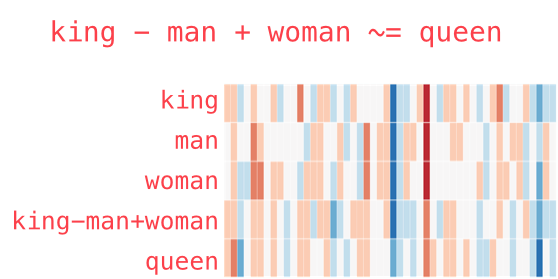
\includegraphics[width=0.9\textwidth]{img/kingmanwomanqueen}
	\captionsource{Subtracting the vectors man from king and adding woman almost results in queen.}{https://jalammar.github.io/illustrated-word2vec/}
	\label{fig:kingmanwomanqueen}
\end{figure}

Two known representatives for word embeddings are \textit{Word2Vec} (\cite{mikolov2013efficient}; \cite{mikolov2013distributed}) and GloVe (\cite{pennington2014glove}). Word2Vec is either trained based on a \textit{continuous bag of words} model (\cite{mikolov2013efficient}, p. 4), predicting a missing word within a sequence, or based on a \textit{skip-gram} model  (\cite{mikolov2013distributed}, p. 2), using a sliding window over a sequence of words. Both approaches for Word2Vec are based on neural networks for learning. GloVe embeddings in contrast are based on matrix factorisation techniques which create embeddings in such a way that the dot product between two embeddings equals the log of their occurrences within a given context (\cite{pennington2014glove}, p. 2; \cite{pennington2014glove}, equation 7). An example of embeddings can be seen in figure \ref{fig:kingmanwomanqueen}, illustrating the embedded information and it's similarity.

These embeddings will have one fixed embedding for each (known) word, independently from their context. We will therefore call these \textit{non-contextualised embeddings}. This implies that for example a word with a meaning dependent on its context will not always be adequately embedded (\cite{young2017recent}, p. 5). Therefore the next step was to use embeddings which are aware of their context. One of these models is Embedding from Language Model (ELMo) (\cite{peters2018deep}), which utilises a bidirectional language model and thereof being aware of words preceding and following the word to embed. We will call these embeddings \textit{contextualised} embeddings.

OpenAI\footnote{https://openai.com/} released their \textit{OpenAI Transformer} (\cite{Radford2018ImprovingLU}) which also creates contextualised embeddings and  provides a pre-trained model to work with. The OpenAI Transformer consists just of the decoder part of the originally released \textit{Transformer} (\cite{vaswani2017attention}). For downstream tasks such as classification, a simple classifier, like a feed-forward network (FFN), can then be used. While transformers achieved remarkable results on previous tasks (\cite{Radford2018ImprovingLU}, p.8), they lost the ability being bi-directional, as ELMo was before.

Bidirectional Encoder Representations from Transformers (BERT), released by Google in May 2019, resolved this problem (\cite{devlin2018bert}), making transformers bidirectional again, using a technique called masking to prevent peeking at the solution.

While all of these models achieve better results than simpler models, they all rely on deep learning and thereby require a lot of computational resources. This report will investigate how much these achievements over the past years can actually be used in a straight-forward task such as sentence classification, by comparing non-contextualised and contextualised word embeddings.

As the computational demand, even for a pre-trained BERT model, is too demanding for the given resources\footnote{Mainly constrained by 16GiBs of memory and 8GiB of video memory.}, DistilBERT (\cite{sanh2019distilbert}) by \textit{Hugging Face}\footnote{https://huggingface.co/} is being used.

\section{Theory}

\textbf{1625 words}

\textit{Present relevant theoretical background, and in particular the models that you have used. Where appropriate, use mathematical formulas.}

For investigating the influence of non-contextualised and contextualised word embeddings, a simple FFN and an LSTM are being used. Additionally, both will be trained once based on non-contextualised word embeddings using Word2Vec and once based on contextualised word embeddings from DistilBERT. For simplicity, we will refer to the FNN and LSTM as models, to Word2Vec as non-contextualised and to (Distil)BERT as contextualised word embeddings interchangeably. Following from that, we will investigate the following four combinations:

\begin{itemize}
    \item FFN (Word2Vec)
    \item LSTM (Word2Vec)
    \item FFN (DistilBERT)
    \item LSTM (DistilBERT)
\end{itemize}

\subsection{Models}

\subsubsection{Feed-Forward Network}

\begin{figure}[hbt]
	\center
	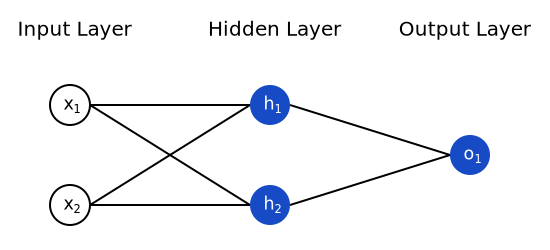
\includegraphics[width=1.0\textwidth]{img/ffn}
	\captionsource{Illustrative feed forward network.}{https://victorzhou.com/blog/intro-to-neural-networks/}
	\label{fig:ffn}
\end{figure}

A FFN consists of multiple layers where the information only flows in one direction. The input is fed to the first layer, which is a linear combination of the inputs and the weights of the first layer. The input will be denoted by $X$ and the weights of the $i$th layer including the bias are denoted by $W_i$. Then, an activation function is applied to map the outback back to a specific range, usually the Sigmoid activation function or a rectified linear (ReLU) function:

\begin{equation}
    \hat{Y_i} = \sigma(X^T W_i)
\end{equation}

This combination is called a dense layer and multiple of those are being stacked and represent the model architecture. The intermediate layers are usually called \textit{hidden} layers as they cannot be directly seen from the outside. Figure \ref{fig:ffn} shows an illustrative FFN. Depending on the desired output, the last activation layer might be skipped. Finally, an error function is being applied to the output. This whole process is called \textit{forward pass}. To update the weights of the model, a \textit{backward pass} is done, which calculates the gradients, as the error depends on the weights. This can be written as:

\begin{equation}
    \nabla E = \left(\frac{\delta E}{\delta W_n}, \frac{\delta E}{\delta W_{n-1}},\: ...\:, \frac{\delta E}{\delta W_1} \right)
\end{equation}

For updating one layer of weights, the partial derivative is being determined. For the last layer, here denoted as $W_n$, the gradient  would look like the following, where $\alpha$ is the \textit{learning rate}:

\begin{equation}
    \frac{\delta E}{\delta W_n} = \frac{\delta E}{\delta \hat{Y}} \frac{\delta \hat{Y}}{\delta A_n} \frac{\delta A_n}{\delta W_n}
\end{equation}

$A_n$ is the intermediate value between the linear combination and the applied activation function. The weights for this layer can then be updated with the following formula:

\begin{equation}
    W_n^{updated} = W_n - \alpha \odot \frac{\delta E}{\delta W_n}
\end{equation}

The remaining layers are updated accordingly, the chain rule just yields in longer equations. Deep neural networks are prone to the vanishing gradient problem (\cite{pascanu2012difficulty}), which can be an issue.

\subsubsection{Long Short-Term Memory}

\begin{figure}[hbt]
	\center
	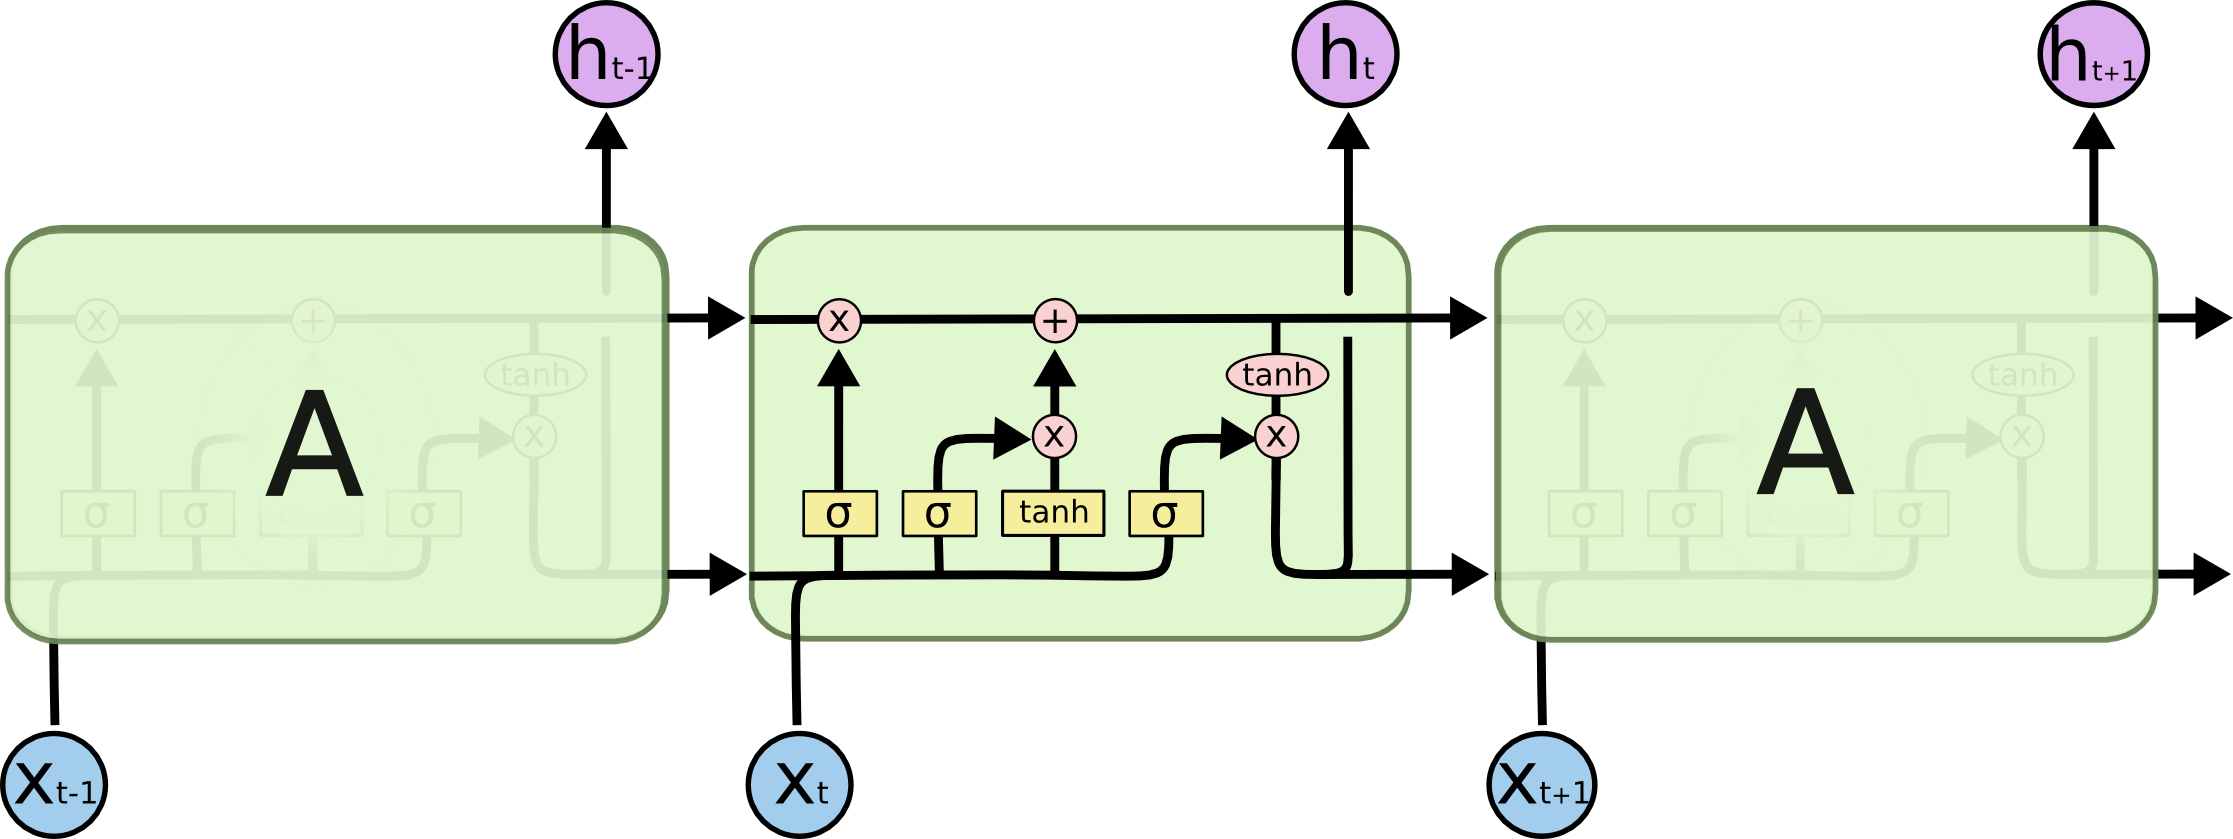
\includegraphics[width=1.0\textwidth]{img/lstm_overview}
	\captionsource{Unfolded LSTM showing the information flow.}{https://colah.github.io/posts/2015-08-Understanding-LSTMs/}
	\label{fig:lstm_overview}
\end{figure}

An LSTM belongs to the field of recurrent neural networks (RNNs) and handles long term relationships better than a classical RNN (\cite{10.1162/neco.1997.9.8.1735,}, abstract). As text can be seen as a sequence with long term dependencies, LSTMs are suitable for catching those long term dependencies. LSTMs, as well as RNNs, look at one element of a sequence (in this context a word) and additionally to the normal output vector, the old cell state is passed on to the next cell handling the second element of the sequence. Utilising this hidden state, information can be preserved and passed on. An unfolded LSTM can be seen in figure \ref{fig:lstm_overview}.
 
In each time step, an LSTM cell sees the Long Term Memory (LTM), denoted as $C_{t-1}$, and the Short Term Memory (STM), denoted as $h_{t-1}$, from the previous cell (previous time step). Additionally, it sees the current element of the sequence, denoted $x_t$. It then produces an output $h_t$, the LTM $C_t$ and the STM $h_t$ for the next cell.
 
This process is enabled by an architecture consisting of four gates, the \textit{forget gate}, the \textit{learn gate}, the \textit{remember gate} and the \textit{use gate}.\footnote{Explanations based on the course "Intro to Deep Learning with PyTorch" on Udacity. Biases have been omitted, as they're included in the weights, variables have been partly renamed to fit the figure. Also https://colah.github.io/posts/2015-08-Understanding-LSTMs/ and the official paper (\cite{10.1162/neco.1997.9.8.1735}) have been used.}
 
\paragraph{Learn Gate} The learn gate takes the new element $x_t$ and concatenates it with the STM ($h_{t-1}$). Then, after taking a linear combination with its weights $W_n$, it passed the results through a \textit{tanh} activation function. This value is denoted as $N_t$. Finally, it is multiplied by an ignore factor $i_t$, making it ignoring unimportant information. The ignore factor is the Sigmoid activation function applied to the linear combination between $W_i$ and the previously concatenated values. The output of the learn gate is thus given as $N_t i_t$ with:
 
\begin{equation}
    N_t = \text{tanh}(W_n(h_{t-1}, x_t)
\end{equation}
 
\begin{equation}
    i_t = \sigma(W_i(h_{t-1}, x_t))
\end{equation}
 
\paragraph{Forget Gate} The forget gate looks at the previous LTM memory $C_{t-1}$ and decides which information is being kept and which is being thrown away. This information is encapsulated in a forget factor $f_t$. The forget factor is the linear combination of the weights $W_f$ multiplied by the concatenated element of the sequence $x_t$ and the previous STM $h_{t-1}$. Afterwards, the Sigmoid activation function is applied. Finally, the output of the forget gate is given as $C_{t-1}f_t$:
 
 \begin{equation}
    f_t = \sigma(W_f(h_{t-1}, x_t))
 \end{equation}
 
\paragraph{Remember Gate} The remember gate looks at the previous LTM $C_{t-1}$ and STM $h_{t-1}$ and then calculates the new LTM state $C_t$, utilising the previously calculated ignore and forget factors $f_t$ and $i_t$:

\begin{equation}
    C_t = C_{t-1}f_t + N_t i_t
\end{equation}
 
\paragraph{Use Gate} The use gate first applies the \textit{tanh} activation function to the linear combination of the weights $W_u$ and the output of the forget gate ($C_{t-1}f_t$) to calculate $U_t$. It then calculates $V_t$ by taking the Sigmoid activation function of the linear combination of $W_v$ and the concatenation of STM $h_{t-1}$ and the current element of the sequence, $x_t$. Then, the output of the use gate is defined as $U_t V_t$.

\begin{equation}
    U_t = \text{tanh}(W_u C_{t-1} f_t)
\end{equation}

\begin{equation}
    V_t = \sigma(W_v (h_{t-1}, E_t))
\end{equation}

The advantage of this architecture is that the previous outputs and hidden states can be treated as fixed variables and the gradient (backward pass) does not depend the whole sequence, mitigating the vanishing gradient problem to some extend. In practice, libraries such as PyTorch, use "reverse-mode automatic differentiation" (\cite{NIPS2019_9015}). Therefore, the calculation of the gradients for an LSTM will not be further investigated.

\subsection{Word Embeddings}

\subsubsection{Word2Vec}

Word2Vec (\cite{mikolov2013efficient}; \cite{mikolov2013distributed}) is being used for the non-contextualised word embeddings. For creating the embeddings, two matrices called the \textit{embedding matrix} and the \textit{context matrix} are being created. Their size also determines the dimensionality of the word embeddings later on. In each learning step, a sample from the embeddings and $n$ negative samples, not occurring in the skip-gram of the original word, are being are taken. This process is called \textit{negative sampling}. The positive sample is looked up in the embeddings matrix, the negatives samples are looked up in the context matrix. Then, the dot product between the positive and each negative sample is being taken (so we have $n$ dot products). As each word embedding has the size $1 \times \text{embedding size}$, the dot product will result in a scalar, to which the Sigmoid activation function is being applied. The result is then compared with the desired output (e.g. 1 for the positive word, 0 for the negative words). Figure \ref{fig:w2v_training_update} illustrates these steps. This whole process is conducted by a neural network, so it is relatively easy to calculate the gradients and to update the weights. The weights, in this case, are the embedding and the context matrices. Once the whole process is completed, the embeddings matrix is being taken as the desired word embeddings. Its size is $\text{number of words} \times \text{embedding size}$. The number of words depends on the corpora and the minimum amount of appearances a word must have.

\begin{figure}[hbt]
	\center
	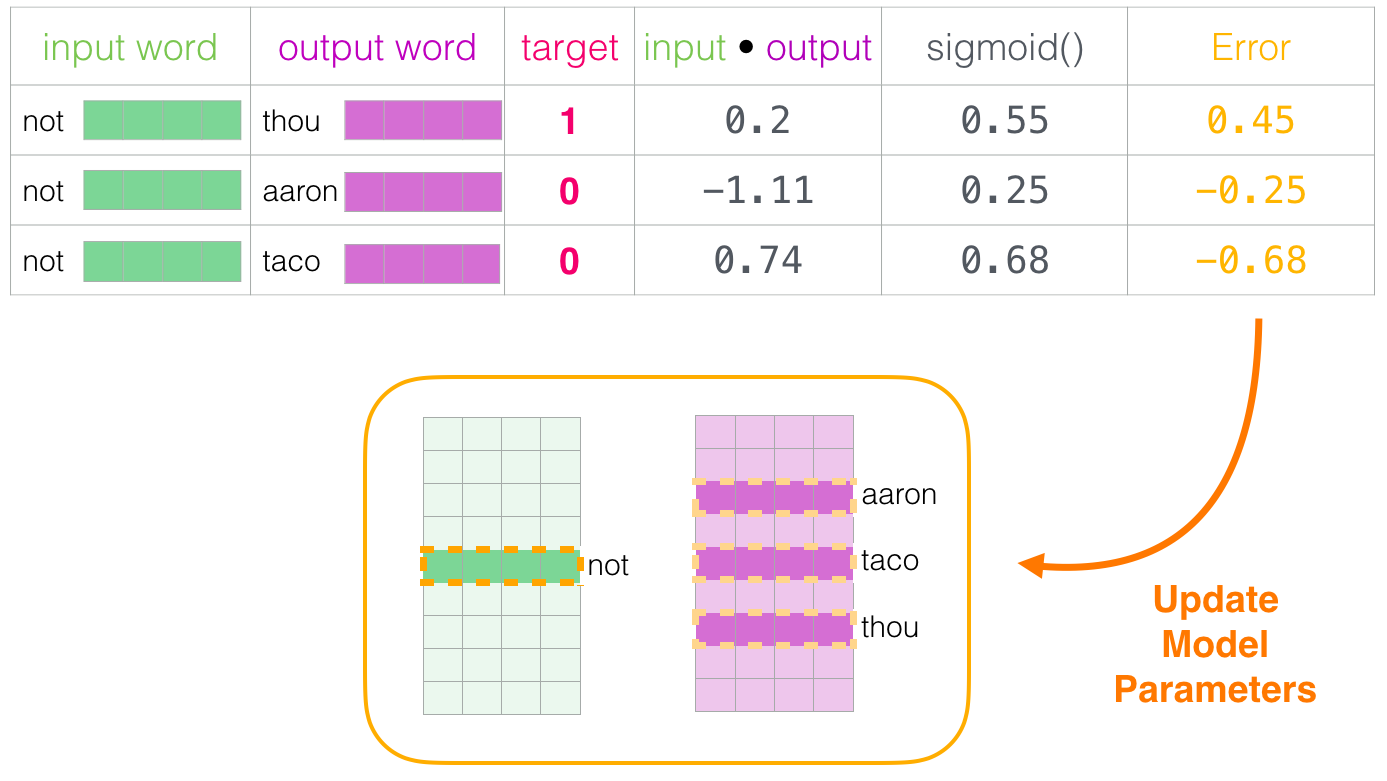
\includegraphics[width=1.0\textwidth]{img/word2vec-training-update.png}
	\captionsource{Training process of Word2Vec embeddings.}{https://jalammar.github.io/illustrated-word2vec/}
	\label{fig:w2v_training_update}
\end{figure}

\subsubsection{BERT}

BERT (\cite{devlin2018bert}) is an encoder based on bidirectional transformer\footnote{Transformers will not be explained in this report as the number of words is quite limited. For a more in-depth understanding, this blog post is recommended: https://jalammar.github.io/illustrated-transformer/}. Transformers use attention heads (\cite{vaswani2017attention}) for focusing on different parts or words of a sentence. For example, if the word \textit{it} is being processed, the attention heads will give focus to different parts of the whole sequence. This way the model can know, which entity is meant by \textit{it}. The advantage is that a sequence is not read from one side to the other, but the whole sequence is processed at once. This is also called \textit{masked LM} or \textit{masked language modeling} (\cite{devlin2018bert}, p. 4).

BERT can unambiguously represent single sentences and pair of two sentences, for example question and answer (\cite{devlin2018bert}, p. 4). Sentences are differentiated by a special \texttt{[SEP]} token. BERT is trained on two tasks: \textit{MLM} (prediction of the real words behind the \texttt{[MASK]} tokens) and Next Sentence Prediction (NSP).

\begin{figure}[hbt]
	\center
	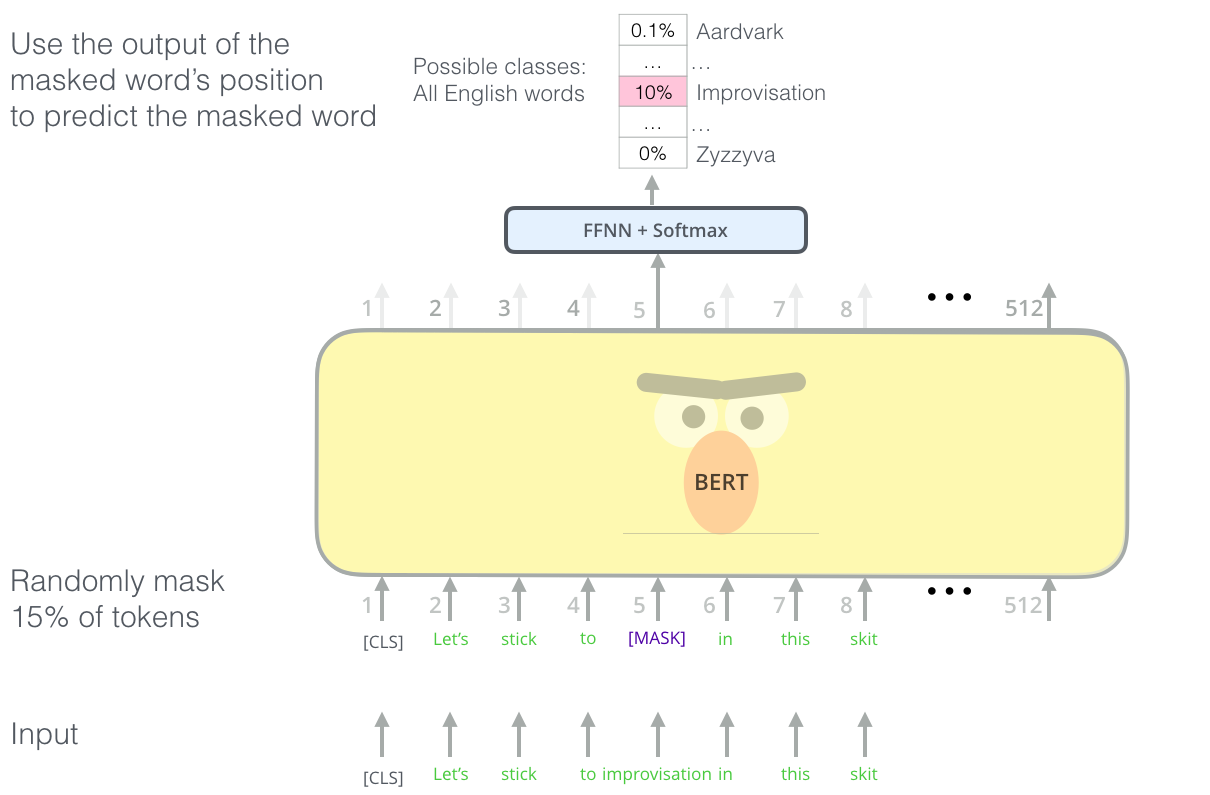
\includegraphics[width=1.0\textwidth]{img/BERT-language-modeling-masked-lm}
	\captionsource{BERT for masked language modeling.}{https://jalammar.github.io/illustrated-bert/}
	\label{fig:bert_mlm}
\end{figure}

\paragraph{MLM} During the training of BERT, before a sequence is passed to BERT, 15 percent of its elements are replaced by special \texttt{[MASK]} tokens, the input is partly shuffled and a special classification token \texttt{[CLS]} is being added at the beginning of the tokenised sentence (\cite{devlin2018bert}, p. 4). BERT then learns to predict the masked tokens. Figure \ref{fig:bert_mlm} illustrates the process.

\begin{figure}[hbt]
	\center
	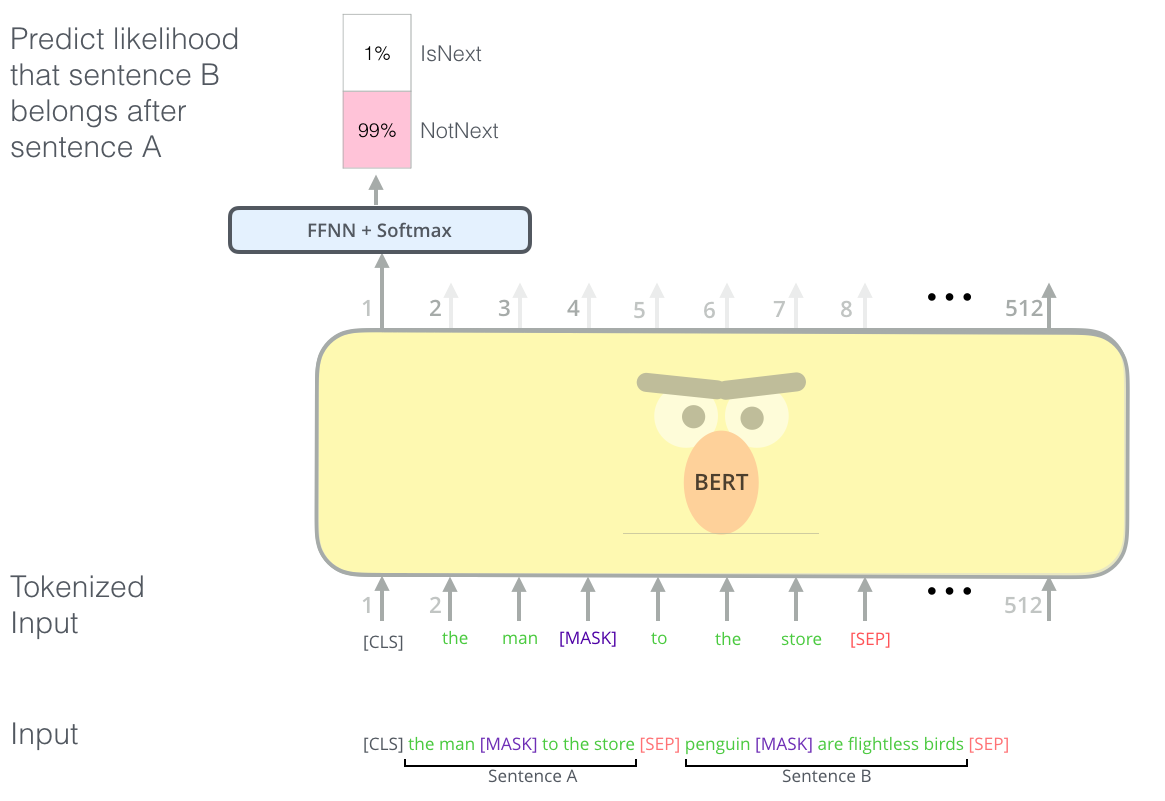
\includegraphics[width=1.0\textwidth]{img/bert-next-sentence-prediction.png}
	\captionsource{Bert for next sentence prediction.}{https://jalammar.github.io/illustrated-bert/}
	\label{fig:bert_nsp}
\end{figure}

\paragraph{NSP} Given two sentences A and B, BERT has to predict the likelihood of sentence B actually following sentence A (\cite{devlin2018bert}, p. 4). Figure \ref{fig:bert_nsp} shows the process.

\begin{figure}[hbt]
	\center
	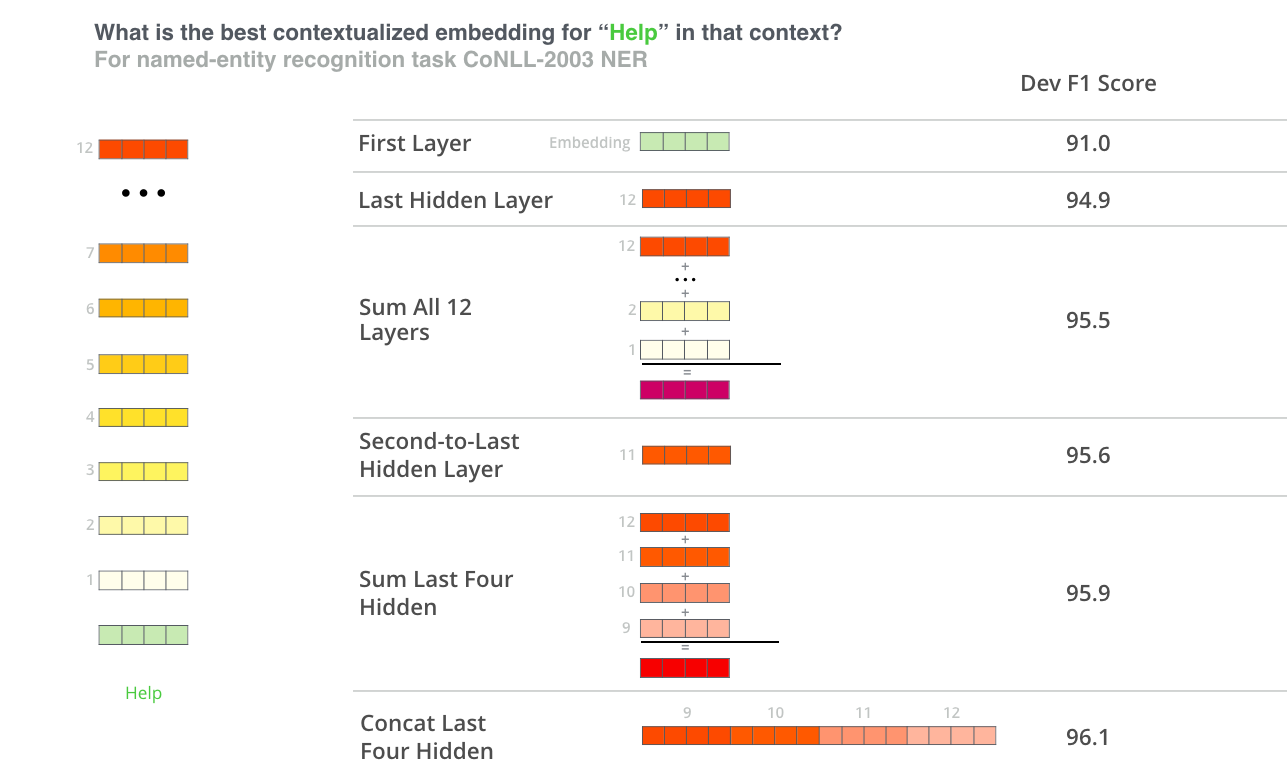
\includegraphics[width=1.0\textwidth]{img/bert-feature-extraction-contextualized-embeddings.png}
	\captionsource{Using BERT for contextualised word embeddings.}{https://jalammar.github.io/illustrated-bert/}
	\label{fig:bert_cwe}
\end{figure}

As BERT is just an encoder, another classifier for downstream tasks such as classification is compulsory. The encoder outputs between the different layers can be used as contextualised word embeddings. Figure \ref{fig:bert_cwe} shows their corresponding $F_1$ scores on the development set during training of BERT. We will use the output of the last encoding layer in this project as embeddings which achieved an $F_1$ score of $94.9$ percent. The specified \texttt{[CLS]} token, originally thought for classification, will not be used as the aim is not to achieve a high accuracy, but rather to compare non-contextualised and contextualised word embeddings.

\subsubsection{DistilBERT}

As even the smallest BERT model has high computational demands, \textit{DistilBERT} (\cite{sanh2019distilbert}) is used for this project. Distillation is a process in which a smaller model tries to mimic the behaviour of a larger model in such a way that it behaves almost the same. The concept was introduced by \cite{10.1145/1150402.1150464} and later generalised by \cite{hinton2015distilling}. The smaller model can also be an enemble of models (similar to the concepts of AdaBoost). The result is a model that is 40 percent smaller and 60 percent faster while keeping 97 percent of BERTs understanding capabilities (\cite{sanh2019distilbert}, p. 5).

\section{Data}

\textbf{339 words}

\subsection{Presentation}

\textit{Present your data. What information does it contain? Where did you get it from? What preprocessing did you do, if any?}

The data set used in this project consists of Amazon reviews categorised by one to five stars and is provided by Xiang Zhang\footnote{http://xzh.me/}. The data is freely available and can be downloaded on Google Drive: \href{https://drive.google.com/drive/folders/0Bz8a\_Dbh9Qhbfll6bVpmNUtUcFdjYmF2SEpmZUZUcVNiMUw1TWN6RDV3a0JHT3kxLVhVR2M}{\texttt{amazon\_review\_full\_csv.tar.gz}}.

Originally, the data is divided into training data with $3\,000\,000$ data points and test data with $650\,000$ data points. Each data point consists of a label, indicating how many stars the review has, a title and the review text. One sample looks like this: \\

\texttt{"3","more like funchuck","Gave this to my dad for a gag gift after directing ""Nunsense,"" he got a reall kick out of it!"} \\

\begin{figure}[hbt]
	\center
	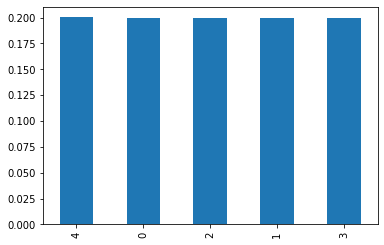
\includegraphics[width=0.6\textwidth]{img/class_distribution}
	\caption{Class distribution.}
	\label{fig:class_distribution}
\end{figure}

\begin{figure}[hbt]
	\center
	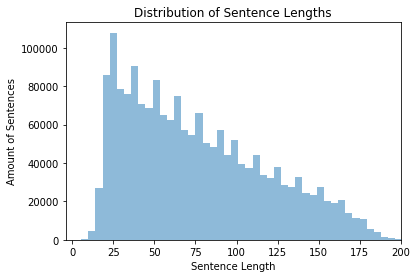
\includegraphics[width=0.6\textwidth]{img/distribution_review_lengths}
	\caption{Distribution of review lengths.}
	\label{fig:review_length_distribution}
\end{figure}

The class distribution can be seen in figure \ref{fig:class_distribution} and the distribution of review lengths (words) can be seen in figure \ref{fig:review_length_distribution}. The percentiles can be found in table \ref{tab:percentiles}.

\begin{table}[h]
    \centering
    \begin{tabular}{l|r|r|r|r|r|r|r|r|r}
         Percentiles & \textbf{91} & \textbf{92} & \textbf{93} & \textbf{94} & \textbf{95} & \textbf{96} & \textbf{97} & \textbf{98} & \textbf{99} \\ \hline
        Review Length & 144 & 147 & 150 & 153 & 157 & 161 & 165 & 170 & 177 \\ 
    \end{tabular}
    \caption{Percentiles and their corresponding reviews lengths.}
    \label{tab:percentiles}
\end{table}

\subsection{Preprocessing}

The original training and test data sets are read, concatenated and shuffled. Then the column for the \textit{title} of the review is being dropped and all labels are shifted by $-1$ so that the labels start at zero: $0, 1, 2, 3 \text{and} 4$. Next, the data is split into 85 percent training, 10 percent validation and 5 percent test data. For the following sentences, a padding of 200 has been used\footnote{Normally only the training data should be used for deciding the padding. Due to time constrains this wasn't changed. As 85 percent randomly chosen data is used for training, the result is likely to not be that much different.}. This lies way above the 99th percentile of $177$ words as it accounts for two facts. Firstly, the sentences become longer due to punctuation, and secondly, some words are being further split during tokenisation.

The padding is applied after tokenisation. The tokeniser used for both, Word2Vec and BERT, is the DistilBERT tokeniser provided by the HuggingFace library\footnote{https://huggingface.co/transformers/model\_doc/distilbert.html\#distilberttokenizer}. For Word2Vec, only the $1\,000\,000$ most common embeddings are taken due to computational constraints. Inferentially, all other word are considered unknown.

After preprocessing, the three data sets are saved as \texttt{.csv} files, where the first $200$ columns hold the word Ids $X$ and the last column holds the label $Y$.

\section{Method}

\textbf{358 words}

\textit{Explain how you carried out your study. Aim to be detailed enough for others to reproduce your results.}

All four model combinations are implemented in PyTorch. The source code and detailed instructions for replicating the results can be found in the corresponding GitHub repository\footnote{https://github.com/flennic/text-mining-project}.

The first step is to create the non-contextualised or contextualised embeddings for the reviews. In the case of Word2Vec, an embedding layer\footnote{https://pytorch.org/docs/stable/nn.html?highlight=embedding\#torch.nn.Embedding} is used, mapping the token Ids to non-contextualised word-embeddings of shape $(200 \times 300)$ where $200$ is the padding length and $300$ the word embedding size of Word2Vec. The embeddings are not frozen, so the embeddings can change during the training process. This is to account for the limitation of not using all Word2Vec embeddings. The embeddings are loaded into the embeddings layer using the Gensim library (\cite{inproceedings}). For the contextualised word embeddings, the tokenised sentences are fed to DistilBERT\footnote{https://huggingface.co/transformers/model\_doc/distilbert.html} and the output of the last encoder is then taken as the embedding. The pretrained model \textit{distilbert-base-uncased} is being used and all weights are frozen during training.

The LSTM directly takes the sequences as input whereas for the FFN the sequences must be flattened first, thus resulting in $60\,000$ inputs. The model parameters can be found in appendix \ref{sec:model_settings} and the architectures are given by the following:

\paragraph{FFN (Word2Vec)} $X$ $\rightarrow$ Embedding $\rightarrow$ Flattening $\rightarrow$ Linear $\rightarrow$ Sigmoid $\rightarrow$ Dropout $\rightarrow$ Linear $\rightarrow$ LogSoftMax

\paragraph{LSTM (Word2Vec)} $X$ $\rightarrow$ Embedding $\rightarrow$ LSTM $\rightarrow$ Dropout $\rightarrow$ Linear $\rightarrow$ Sigmoid $\rightarrow$ LogSoftMax

\paragraph{FFN (DistilBERT)} $X$ $\rightarrow$ DistilBERT $\rightarrow$ Flattening $\rightarrow$ Linear $\rightarrow$ Sigmoid $\rightarrow$ Dropout $\rightarrow$ Linear $\rightarrow$ LogSoftMax

\paragraph{LSTM (DistilBERT)} $X$ $\rightarrow$ DistilBERT $\rightarrow$ LSTM $\rightarrow$ Dropout $\rightarrow$ Linear $\rightarrow$ Sigmoid $\rightarrow$ LogSoftMax \\

The last linear layer is always used to map to the five classes of Amazon reviews, thus the labels. Furthermore, dropout (\cite{JMLR:v15:srivastava14a}) is being applied for regularisation and the gradients for the LSTM are clipped at a value of $5$ to prevent exploding gradients (\cite{pascanu2012difficulty}). Adam (\cite{kingma2014adam}) is used as the optimiser and cross-entropy loss as the loss function.

As the data set is balanced, the measurement being used is accuracy since it provides a single value to adequately estimate the performance of the models.

\section{Results}

\textbf{397 words}

\textit{Present your results in an objective way. Use tables and charts, but do not forget to also include a summary in text form. Do not interpret your results.}

All four model combinations and their achieved accuracies can be seen in table \ref{tab:results}. The accuracies for training have dropout enabled\footnote{Enabling another prediction without dropout would have been too time consuming for this project.} and are trailing accuracies. This means that the accuracy will jump between the epochs, as the model is usually less accurate during the beginning of an epoch and the trailing training accuracy is always the average up to the current batch. Figure \ref{fig:ffn_w2v_results} shows the accuracies for the FFN with Word2Vec embeddings for training, validation and test for different epochs, figure \ref{fig:ffn_bert_results} shows the accuracies for the FFN with DistilBERT, figure \ref{fig:lstm_w2v_results} shows the accuracies for the LSTM with Word2Vec embeddings and figure \ref{fig:lstm_bert_results} shows the accuracies for the LSTM with DestilBERT embeddings. The lowest baseline accuracy is around $20.00$ percent which could be achieved by simply predicting one class at all times.

\begin{table}[h]
    \centering
    \begin{tabular}{l|r|r|r}
        Model | Data & \textbf{Training} & \textbf{Validation} & \textbf{Testing} \\ \hline
        FFN (W2V) & 52.80\% & 52.82\% & 43.10\% \\ 
        FFN (BERT) & 49.88\% & 49.88\% & 49.98\% \\
        LSTM (W2V) & 50.14\% & 50.08\% & 50.49\% \\
        LSTM (BERT) & 56.13\% & 56.14\% & 56.43\% \\
    \end{tabular}
    \caption{Highest accuracies for the different setups. Note that training has dropout enabled.}
    \label{tab:results}
\end{table}

It can be seen that the FFN with Word2Vec embeddings has the lowest testing score with a test accuracy of $43.10$ percent. The FFN using DistilBERT embeddings achieves a higher test accuracy of $49.98$ percent, closely followed by the LSTM using Word2Vec embeddings with a test accuracy of $50.49$ percent. The highest accuracy is achieved by the LSTM in combination with DistilBERT embeddings and peaks at $56.43$ for the test data set. For all model combinations, except the FFN using Word2Vec embeddings, the test accuracy is slightly higher compared to their validation accuracies, which seems a bit odd. This pattern can be seen for all these other models. For the FFN, using Word2Vec, the test accuracy is way lower than the training or validation accuracy\footnote{Due to these results the source code has been investigated but no issues have been found. Therefore these results are treated as valid.}.

\begin{figure}[hbt]
	\center
	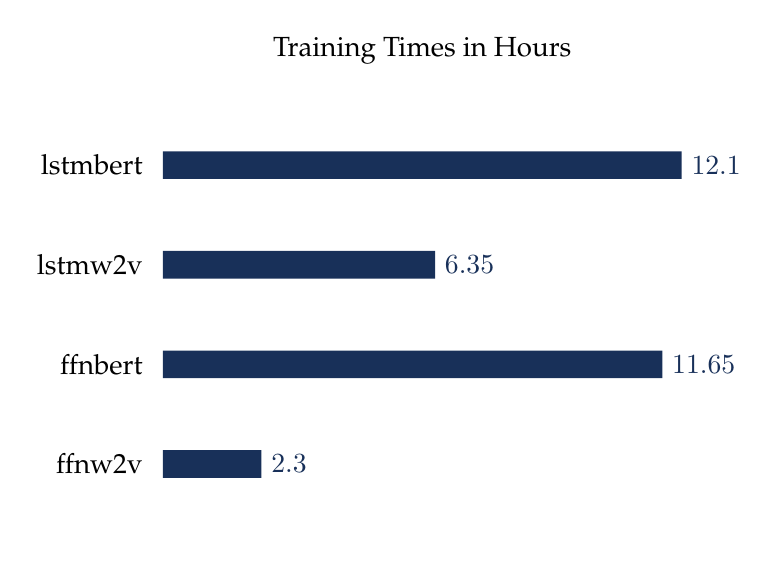
\begin{tikzpicture}
          \begin{axis}[title = Training Times in Hours,
            xbar,
            y axis line style = { opacity = 0 },
            axis x line       = none,
            tickwidth         = 0pt,
            xmin              = 0,
            enlarge y limits  = 0.25,
            enlarge x limits  = 0.02,
            symbolic y coords = {ffnw2v,ffnbert,lstmw2v,lstmbert},
            nodes near coords,
            %cycle list name=exotic,
            legend style={at={(1.335,1)},anchor=north east},
            every axis plot/.append style={fill,draw=none,no markers}
          ]
          \addplot[color=custom_five] coordinates {(2.3,ffnw2v)
                                (11.65,ffnbert)
                                (6.35,lstmw2v)
                                (12.1,lstmbert)};
          \end{axis}
        \end{tikzpicture}
	\caption{Training times for the different model combinations.}
	\label{fig:training_times}
\end{figure}

Figure \ref{fig:training_times} shows the training times for the model combinations. The models using non-contextualised word embeddings (Word2Vec) are trained for 30 epochs and the models using contextualised word embeddings (DistilBERT) are trained for 3 epochs. Both models using DistilBERT word embeddings have the highest training times with $12.1$ hours for the LSTM and and $11.65$ hours for the FFN. Around half of the time is needed for the LSTM with Word2Vec word embeddings with a training time around $6.35$ hours. The lowest training time is achieved by the FFN with Word2Vec embeddings and takes just $2.3$ hours.

% ffn_w2v
\begin{figure}[hbt]
	\center
	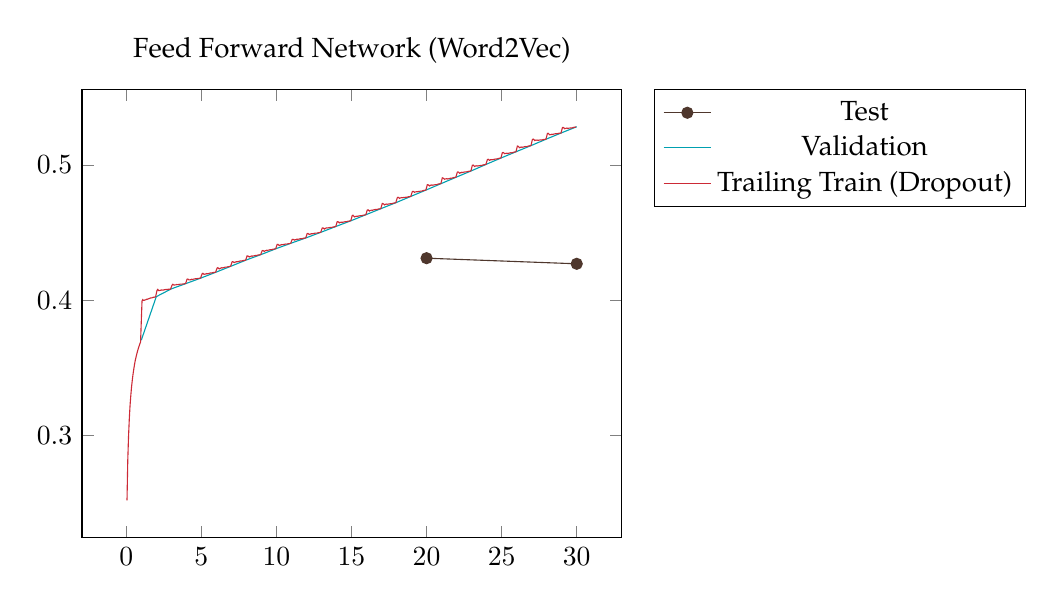
\begin{tikzpicture}
      \begin{axis}[
      title = Feed Forward Network (Word2Vec),
      legend style={at={(1.75,1)},anchor=north east},
      ]
        \legend{Test, Validation, Trailing Train (Dropout)}
        
        % test_ffn_w2v
        \addplot[mark=*, color=custom_four] coordinates {(20, 0.4310301369863014) (30, 0.42688219178082193)};
        
        % validation_ffn_w2v
        \addplot[mark=none,color=custom_one] coordinates {
            (1, 0.3704028203062047)
            (2, 0.4026007252215955)
            (3, 0.4083515713134569)
            (4, 0.41237824335213535)
            (5, 0.4164758259468171)
            (6, 0.4207989524576954)
            (7, 0.4252283642224013)
            (8, 0.42973199033037873)
            (9, 0.43381555197421434)
            (10, 0.4381569701853344)
            (11, 0.44219911361805)
            (12, 0.4461583400483481)
            (13, 0.45032586623690574)
            (14, 0.45462949234488315)
            (15, 0.4588535052377115)
            (16, 0.4633323932312651)
            (17, 0.46781901692183725)
            (18, 0.4722376309427881)
            (19, 0.4769203062046736)
            (20, 0.481549556809025)
            (21, 0.4862997582594682)
            (22, 0.49100652699435937)
            (23, 0.4956659951651894)
            (24, 0.5005204673650282)
            (25, 0.5052651087832393)
            (26, 0.5098707493956487)
            (27, 0.5144355358581789)
            (28, 0.5191511684125705)
            (29, 0.5237181305398871)
            (30, 0.5281663174858985)
        };
        
        % training_ffn_w2v_dict
        \addplot[mark=none,color=custom_three] coordinates {
            (0.05, 0.2520703767475329)
            (0.1, 0.28129015470805924)
            (0.151, 0.2990139074492873)
            (0.201, 0.3118442736173931)
            (0.251, 0.3218004728618421)
            (0.301, 0.3292616459361294)
            (0.35100000000000003, 0.33575990146264095)
            (0.401, 0.34083255968595805)
            (0.452, 0.34529943633497806)
            (0.502, 0.34909475226151315)
            (0.552, 0.35259206671463816)
            (0.602, 0.3555636489600466)
            (0.652, 0.35800195609027075)
            (0.7020000000000001, 0.36024130914444313)
            (0.753, 0.36240212959155704)
            (0.8029999999999999, 0.36434755827251236)
            (0.853, 0.36601876179131193)
            (0.903, 0.36768167060718204)
            (0.953, 0.36914958584011426)
            (1.05, 0.3994028191817434)
            (1.1, 0.40041953638980265)
            (1.151, 0.39981507418448464)
            (1.201, 0.3999127839740954)
            (1.251, 0.4001558002672697)
            (1.301, 0.40025784676535087)
            (1.351, 0.4006829512746711)
            (1.401, 0.40069037989566203)
            (1.452, 0.40091067308570905)
            (1.502, 0.40108305278577305)
            (1.552, 0.4013355017849133)
            (1.6019999999999999, 0.4015703703227796)
            (1.6520000000000001, 0.401648764668206)
            (1.702, 0.4017145830885808)
            (1.7530000000000001, 0.4019374914336623)
            (1.803, 0.40213604977256373)
            (1.853, 0.40217708434113775)
            (1.903, 0.40233206051832054)
            (1.9529999999999998, 0.4024927028328428)
            (2.05, 0.40729081003289475)
            (2.1, 0.40799753289473684)
            (2.151, 0.4071226956551535)
            (2.201, 0.4070779900801809)
            (2.251, 0.4072766755756579)
            (2.301, 0.40734033417283444)
            (2.351, 0.40756684496886747)
            (2.401, 0.4074291430021587)
            (2.452, 0.40750175609923245)
            (2.502, 0.4075579191509046)
            (2.552, 0.40771907824648623)
            (2.602, 0.4078473542865954)
            (2.652, 0.4078729915232793)
            (2.702, 0.40783496369096567)
            (2.753, 0.40795759234512063)
            (2.803, 0.4080808539139597)
            (2.8529999999999998, 0.4080673548459269)
            (2.903, 0.4081610964055647)
            (2.953, 0.4082677106778047)
            (3.05, 0.41112960012335525)
            (3.1, 0.411751998098273)
            (3.151, 0.41126666152686403)
            (3.201, 0.4111565037777549)
            (3.251, 0.41129503752055924)
            (3.301, 0.41130788702713816)
            (3.351, 0.41161283335291354)
            (3.401, 0.41145224320261103)
            (3.452, 0.41156844646610014)
            (3.502, 0.4116029438219572)
            (3.552, 0.4117057836797249)
            (3.602, 0.4118373937774123)
            (3.652, 0.41186029225708504)
            (3.702, 0.41183437261366307)
            (3.753, 0.4119617127535636)
            (3.803, 0.41209090383429275)
            (3.8529999999999998, 0.41204815088041796)
            (3.903, 0.4121721948099415)
            (3.953, 0.41228808458492033)
            (4.05, 0.41553537469161184)
            (4.1, 0.4156213057668586)
            (4.151, 0.4150990268640351)
            (4.201, 0.4149607608192845)
            (4.251, 0.41508853310032895)
            (4.301, 0.41502433910704495)
            (4.351, 0.41547548681273494)
            (4.401, 0.41531251606188324)
            (4.452, 0.41547969349643643)
            (4.502, 0.4155604312294408)
            (4.552, 0.41576535165595097)
            (4.602, 0.4158141822145696)
            (4.652, 0.4158442570612981)
            (4.702, 0.41585753017798405)
            (4.753, 0.41599763569078946)
            (4.803, 0.4161598807887027)
            (4.853, 0.4161505448190789)
            (4.9030000000000005, 0.41628376921715093)
            (4.953, 0.41637050808301596)
            (5.05, 0.41949141652960525)
            (5.1, 0.4198407624897204)
            (5.151, 0.4192617315995066)
            (5.201, 0.4191384566457648)
            (5.251, 0.41936003032483554)
            (5.301, 0.41935917369106357)
            (5.351, 0.4196671794231673)
            (5.401, 0.41944543938887746)
            (5.452, 0.419636687340095)
            (5.502, 0.4197557951274671)
            (5.552, 0.41993151212993424)
            (5.602, 0.42010243733723956)
            (5.652, 0.42010559823348936)
            (5.702, 0.4201533955738957)
            (5.753, 0.4202833744517544)
            (5.803, 0.42044599432694285)
            (5.853, 0.42045560193135645)
            (5.9030000000000005, 0.42058871085183663)
            (5.953, 0.42071854440789475)
            (6.05, 0.42374460320723684)
            (6.1, 0.42406262849506576)
            (6.151, 0.4234437105948465)
            (6.201, 0.42313585783305924)
            (6.251, 0.4235663163034539)
            (6.301, 0.4236268160635965)
            (6.351, 0.42397543541470867)
            (6.401, 0.4237821478592722)
            (6.452, 0.4240074826959978)
            (6.502, 0.4240865607010691)
            (6.552, 0.4242888090142793)
            (6.602, 0.4244592231616639)
            (6.652, 0.4244280981148785)
            (6.702, 0.42446348720923405)
            (6.753, 0.4246483518366228)
            (6.803, 0.42479956777472244)
            (6.853, 0.42483170925648217)
            (6.9030000000000005, 0.4249938607913012)
            (6.953, 0.4251161189620845)
            (7.05, 0.42834312037417765)
            (7.1, 0.42844350714432566)
            (7.151, 0.4280165287486294)
            (7.201, 0.4278126766807155)
            (7.251, 0.42817671926398027)
            (7.301, 0.42818303693804827)
            (7.351, 0.42850442757283835)
            (7.401, 0.42838066502621297)
            (7.452, 0.4285597773323282)
            (7.502, 0.428628218801398)
            (7.552, 0.4288284812817733)
            (7.602, 0.4289805094401042)
            (7.652, 0.428953101277834)
            (7.702, 0.4290158838257754)
            (7.753, 0.42919150904605263)
            (7.803, 0.42933343586168793)
            (7.853, 0.42932204491582815)
            (7.9030000000000005, 0.4294894034402412)
            (7.953, 0.4296038936710094)
            (8.05, 0.4327537135074013)
            (8.1, 0.4326758133737664)
            (8.151, 0.43222206517269735)
            (8.201, 0.4318807501541941)
            (8.251, 0.4323434930098684)
            (8.301, 0.4323604650664748)
            (8.351, 0.43268808924165886)
            (8.401, 0.4324955187345806)
            (8.452, 0.4326898229052449)
            (8.502, 0.4326944451583059)
            (8.552, 0.43288556696695574)
            (8.602, 0.43303546570895013)
            (8.652, 0.43299859545008856)
            (8.702, 0.4330759837215108)
            (8.753, 0.43326608758223684)
            (8.803, 0.43342961763080795)
            (8.853, 0.4334321863511029)
            (8.903, 0.43360035321865864)
            (8.953, 0.433703647095741)
            (9.05, 0.43650095086348684)
            (9.1, 0.4367242110402961)
            (9.151, 0.43633230108963816)
            (9.201, 0.43599660773026316)
            (9.251, 0.4365478515625)
            (9.301, 0.4365908974095395)
            (9.351, 0.43688345313968513)
            (9.401, 0.4367679796720806)
            (9.452, 0.4369567514163012)
            (9.502, 0.43702922620271384)
            (9.552, 0.4372341028240879)
            (9.602, 0.43738970840186403)
            (9.652, 0.43729860869496456)
            (9.702, 0.43738481335173873)
            (9.753, 0.4375719572368421)
            (9.803, 0.4377202485737048)
            (9.853, 0.4377515101949497)
            (9.903, 0.43793144002992507)
            (9.953, 0.43802556172632445)
            (10.05, 0.4412183259662829)
            (10.1, 0.44129140753495066)
            (10.151, 0.4407273677357456)
            (10.201, 0.44038230494449015)
            (10.251, 0.44080489309210524)
            (10.301, 0.4408033939830044)
            (10.351, 0.44111782446839753)
            (10.401, 0.4410097222579153)
            (10.452, 0.44112945021244515)
            (10.502, 0.44117544073807563)
            (10.552, 0.4413443387410287)
            (10.602, 0.4414829454923931)
            (10.652, 0.44142886018946104)
            (10.702, 0.441472447904429)
            (10.753, 0.44161773146244515)
            (10.803, 0.44175358822471217)
            (10.853, 0.4417406206160507)
            (10.903, 0.44191443013866044)
            (10.953, 0.4420683377337258)
            (11.05, 0.4448724043996711)
            (11.1, 0.444985640676398)
            (11.151, 0.4447556880482456)
            (11.201, 0.4443704705489309)
            (11.251, 0.44469411749588816)
            (11.301, 0.4446553012780976)
            (11.351, 0.4450380712523496)
            (11.401, 0.4450011002390008)
            (11.452, 0.4450628269485563)
            (11.502, 0.44513405247738486)
            (11.552, 0.44530855753775417)
            (11.602, 0.44546294630619515)
            (11.652, 0.4453750177916245)
            (11.702, 0.44543399667381345)
            (11.753, 0.4456053616707785)
            (11.803, 0.44575781571237666)
            (11.853, 0.44576478373524575)
            (11.903, 0.44591999611659355)
            (11.953, 0.44604788064296225)
            (12.05, 0.4492235685649671)
            (12.1, 0.449301468698602)
            (12.151, 0.44881987989994515)
            (12.201, 0.44854736328125)
            (12.251, 0.4488959061472039)
            (12.301, 0.44886164079632673)
            (12.351, 0.44919534554158835)
            (12.401, 0.4490611427708676)
            (12.452, 0.44921071905838816)
            (12.502, 0.4492988987972862)
            (12.552, 0.4494666870701256)
            (12.602, 0.4495701036955181)
            (12.652, 0.44952627328725964)
            (12.702, 0.44957509435209114)
            (12.753, 0.44976303368283993)
            (12.803, 0.4499365154065584)
            (12.853, 0.44991611917690594)
            (12.903, 0.4500970673142818)
            (12.953, 0.4502124733541811)
            (13.05, 0.4532615260074013)
            (13.1, 0.4534502531352796)
            (13.151, 0.4529799076548794)
            (13.201, 0.4525764866879112)
            (13.251, 0.45311986019736844)
            (13.301, 0.45322993763706143)
            (13.351, 0.4534730839550047)
            (13.401, 0.4533546849300987)
            (13.452, 0.45347479212353803)
            (13.502, 0.4535630075555099)
            (13.552, 0.4536671615673594)
            (13.602, 0.45381753486499454)
            (13.652, 0.4537580853049089)
            (13.702, 0.45381497261219456)
            (13.753, 0.4540111876370614)
            (13.803, 0.4541799645674856)
            (13.853, 0.4542250500374903)
            (13.903, 0.4543461492884229)
            (13.953, 0.45446836519109246)
            (14.05, 0.45806081671463816)
            (14.1, 0.4580527857730263)
            (14.151, 0.45760144685444076)
            (14.201, 0.4570641768606086)
            (14.251, 0.4575635408100329)
            (14.301, 0.45750989412006576)
            (14.351, 0.45767257805157424)
            (14.401, 0.4575297707005551)
            (14.452, 0.4576558787920322)
            (14.502, 0.45779226202713813)
            (14.552, 0.45793684817957536)
            (14.602, 0.4580739339192708)
            (14.652, 0.4579940981227859)
            (14.702, 0.45809592340225563)
            (14.753, 0.45832337496573466)
            (14.803, 0.4584584487111945)
            (14.853, 0.45846236379523025)
            (14.903, 0.45862101950840645)
            (14.953, 0.45875342202648894)
            (15.05, 0.46255171926398025)
            (15.1, 0.46277819181743424)
            (15.151, 0.4620923494037829)
            (15.201, 0.4615241602847451)
            (15.251, 0.461920166015625)
            (15.301, 0.46187364009388704)
            (15.351, 0.4620503590519267)
            (15.401, 0.4619636535644531)
            (15.452, 0.4621269716853984)
            (15.502, 0.4622505589535362)
            (15.552, 0.4623519678435257)
            (15.602, 0.46249336108826755)
            (15.652, 0.4624245832806174)
            (15.702, 0.46247416331355734)
            (15.753, 0.4626720763089364)
            (15.803, 0.4628488641036184)
            (15.853, 0.46287569689676855)
            (15.903, 0.46303705583538923)
            (15.953, 0.4631657058842625)
            (16.05, 0.4665157920435855)
            (16.1, 0.46679526881167765)
            (16.151, 0.46625933730811403)
            (16.201, 0.46585404245476975)
            (16.251, 0.4662992778577303)
            (16.301, 0.4663822107147752)
            (16.351, 0.46655617620711937)
            (16.401, 0.4664411042865954)
            (16.452, 0.46665463810078583)
            (16.502, 0.4668111700760691)
            (16.552, 0.4669163170043361)
            (16.602, 0.4670788948996025)
            (16.652, 0.4670123513410931)
            (16.702, 0.4670602898848684)
            (16.753, 0.4672572085731908)
            (16.803, 0.4674074273360403)
            (16.853, 0.467455128767173)
            (16.903, 0.4675565128437957)
            (16.953, 0.46766548473749137)
            (17.05, 0.4714853387129934)
            (17.1, 0.4713600560238487)
            (17.151, 0.4709424470600329)
            (17.201, 0.47042565596731084)
            (17.251, 0.47083675986842105)
            (17.301, 0.4709014892578125)
            (17.351, 0.47103285251703475)
            (17.401, 0.47089586759868424)
            (17.452, 0.4710302520216557)
            (17.502, 0.4711019415604441)
            (17.552, 0.47120805220170453)
            (17.602, 0.47133234927528783)
            (17.652, 0.4712892601847166)
            (17.702, 0.47134938634427864)
            (17.753, 0.4715697171395285)
            (17.803, 0.47174192729749176)
            (17.853, 0.4718135680207527)
            (17.903, 0.4719597888968841)
            (17.953, 0.47209027995693387)
            (18.05, 0.47568712736430924)
            (18.1, 0.4760918868215461)
            (18.151, 0.47568659196820173)
            (18.201, 0.4751944290964227)
            (18.251, 0.4756276983963816)
            (18.301, 0.4756496496367873)
            (18.351, 0.47583053703594924)
            (18.401, 0.47570620085063736)
            (18.452, 0.4758420353047332)
            (18.502, 0.47589304070723687)
            (18.552, 0.4759771173650568)
            (18.602, 0.4760467796994929)
            (18.652, 0.4760073766051999)
            (18.702, 0.47607467766094924)
            (18.753, 0.476299834669682)
            (18.803, 0.4764531788073088)
            (18.853, 0.4764869146671827)
            (18.903, 0.476615325749269)
            (18.953, 0.4767535518741344)
            (19.05, 0.4801748175370066)
            (19.1, 0.48044546026932566)
            (19.151, 0.4801111054002193)
            (19.201, 0.47968493009868424)
            (19.251, 0.4800048828125)
            (19.301, 0.48006613212719296)
            (19.351, 0.48021084204652253)
            (19.401, 0.4801280373021176)
            (19.452, 0.48033829181514986)
            (19.502, 0.48040883917557564)
            (19.552, 0.48044363505532295)
            (19.602, 0.48062321177700107)
            (19.652, 0.4805757468528593)
            (19.702, 0.48067239173372883)
            (19.753, 0.48092212342379387)
            (19.803, 0.4810769934403269)
            (19.853, 0.48111311496226783)
            (19.903, 0.4812666686654788)
            (19.953, 0.4813916319955419)
            (20.05, 0.4853258634868421)
            (20.1, 0.48534995631167765)
            (20.151, 0.4848836263020833)
            (20.201, 0.4844255949321546)
            (20.251, 0.48495644017269735)
            (20.301, 0.48487693385074015)
            (20.351, 0.485198974609375)
            (20.401, 0.4849753128854852)
            (20.452, 0.48504638671875)
            (20.502, 0.48519222861842104)
            (20.552, 0.48528439462470097)
            (20.602, 0.48542772259628564)
            (20.652, 0.48539134654921556)
            (20.702, 0.48546284840519266)
            (20.753, 0.48572002210115134)
            (20.803, 0.48587999845805924)
            (20.853, 0.4859571899791989)
            (20.903, 0.486051146747076)
            (20.953, 0.48618356805098684)
            (21.05, 0.49044639185855265)
            (21.1, 0.49020546361019735)
            (21.151, 0.4897878546463816)
            (21.201, 0.4893903230365954)
            (21.251, 0.48962980571546055)
            (21.301, 0.4897005850808662)
            (21.351, 0.48983994103912126)
            (21.401, 0.48955596120733963)
            (21.452, 0.4896823816132127)
            (21.502, 0.4898488898026316)
            (21.552, 0.48996745570424644)
            (21.602, 0.4901578133566338)
            (21.652, 0.49009661346311995)
            (21.702, 0.4902269176970747)
            (21.753, 0.49043386358963814)
            (21.803, 0.4906241768284848)
            (21.853, 0.4906744706003289)
            (21.903, 0.4907811036583973)
            (21.953, 0.49091379266036184)
            (22.05, 0.49466906095805924)
            (22.1, 0.4947943436472039)
            (22.151, 0.4944024336965461)
            (22.201, 0.49379529451069076)
            (22.251, 0.494140625)
            (22.301, 0.4941912199321546)
            (22.351, 0.49453138767328475)
            (22.401, 0.4943697076094778)
            (22.452, 0.4945366396541484)
            (22.502, 0.4946599056846217)
            (22.552, 0.49471651652212917)
            (22.602, 0.4948644805372807)
            (22.652, 0.49483289216694076)
            (22.702, 0.4949273130947486)
            (22.753, 0.49512414764939694)
            (22.803, 0.49523433886076274)
            (22.853, 0.4952803573372194)
            (22.903, 0.4954074614229258)
            (22.953, 0.4955298933626212)
            (23.05, 0.4997301603618421)
            (23.1, 0.49985062448601975)
            (23.151, 0.4992761444627193)
            (23.201, 0.49882667943050985)
            (23.251, 0.49919947574013157)
            (23.301, 0.49918566252055924)
            (23.351, 0.4993449046199483)
            (23.401, 0.499154341848273)
            (23.452, 0.49923920213130485)
            (23.502, 0.4993965550472862)
            (23.552, 0.49946645344273327)
            (23.602, 0.49956284907826204)
            (23.652, 0.49951666086791496)
            (23.702, 0.49963826344425516)
            (23.753, 0.4998879951343202)
            (23.803, 0.5000350349827817)
            (23.853, 0.5001106380309114)
            (23.903, 0.5002432482981543)
            (23.953, 0.5003569119524758)
            (24.05, 0.5038789447985197)
            (24.1, 0.5041929546155428)
            (24.151, 0.5037274277001097)
            (24.201, 0.5033027247378701)
            (24.251, 0.50380859375)
            (24.301, 0.5037397418105811)
            (24.351, 0.5039296544584116)
            (24.401, 0.5037847820081209)
            (24.452, 0.5040083321911549)
            (24.502, 0.5041192305715461)
            (24.552, 0.5041987222917913)
            (24.602, 0.5042994984409266)
            (24.652, 0.5042812331967991)
            (24.702, 0.5043799608273614)
            (24.753, 0.5046306409333882)
            (24.803, 0.5047922636333265)
            (24.853, 0.5048733643333978)
            (24.903, 0.5049979226631031)
            (24.953, 0.5051039592711218)
            (25.05, 0.5090797825863487)
            (25.1, 0.5091359991776315)
            (25.151, 0.5087553325452303)
            (25.201, 0.5082738775956003)
            (25.251, 0.5084893477590461)
            (25.301, 0.5084359687671327)
            (25.351, 0.5086649270882284)
            (25.401, 0.5084029749820107)
            (25.452, 0.5084942377101608)
            (25.502, 0.5087101986533717)
            (25.552, 0.508783659866552)
            (25.602, 0.508931879411664)
            (25.652, 0.5088966771175987)
            (25.702, 0.508974003612547)
            (25.753, 0.5091803299753289)
            (25.803, 0.5093463094610917)
            (25.853, 0.5094522293138061)
            (25.903, 0.509569045395879)
            (25.953, 0.509698756844053)
            (26.05, 0.5139095908717105)
            (26.1, 0.513759412263569)
            (26.151, 0.5131996556332237)
            (26.201, 0.5126495361328125)
            (26.251, 0.5130213687294408)
            (26.301, 0.512965955232319)
            (26.351, 0.5131936897908834)
            (26.401, 0.5130081176757812)
            (26.452, 0.5131746704815424)
            (26.502, 0.5133507979543586)
            (26.552, 0.5134449643951854)
            (26.602, 0.513531199672766)
            (26.652, 0.5134813563543775)
            (26.702, 0.5135426915677866)
            (26.753, 0.5138146116022478)
            (26.803, 0.5139800623843545)
            (26.853, 0.5140747448239165)
            (26.903, 0.514139721965232)
            (26.953, 0.514283071924775)
            (27.05, 0.5187940095600329)
            (27.1, 0.5190758956106085)
            (27.151, 0.5187062045984101)
            (27.201, 0.5179579885382402)
            (27.251, 0.5183127955386513)
            (27.301, 0.5181750916598136)
            (27.351, 0.5183507015830592)
            (27.401, 0.518139688592208)
            (27.452, 0.5181779471057201)
            (27.502, 0.5182862934313323)
            (27.552, 0.5183726041510915)
            (27.602, 0.5184422543174342)
            (27.652, 0.5183855435143598)
            (27.702, 0.5184378946634164)
            (27.753, 0.5186092979029605)
            (27.803, 0.5187823646946957)
            (27.853, 0.5187938205967009)
            (27.903, 0.5188885962056835)
            (27.953, 0.518969760376991)
            (28.05, 0.5232431512129935)
            (28.1, 0.523372449372944)
            (28.151, 0.5227377372875548)
            (28.201, 0.522186279296875)
            (28.251, 0.5223867315995065)
            (28.301, 0.5223974930612665)
            (28.351, 0.5226676768826363)
            (28.401, 0.5224757947419819)
            (28.452, 0.5226354766310307)
            (28.502, 0.5228412828947369)
            (28.552, 0.5229300905072518)
            (28.602, 0.5230299297131991)
            (28.652, 0.5229515662560096)
            (28.702, 0.5230116306390977)
            (28.753, 0.5231919673451206)
            (28.803, 0.5233544801410875)
            (28.853, 0.5233976287369388)
            (28.903, 0.5234125148483187)
            (28.953, 0.5235378445020343)
            (29.05, 0.5275621916118421)
            (29.1, 0.527666593852796)
            (29.151, 0.527258086622807)
            (29.201, 0.5267177381013569)
            (29.251, 0.5269383480674342)
            (29.301, 0.5269609417831689)
            (29.351, 0.5272308579064849)
            (29.401, 0.5269277472245065)
            (29.452, 0.527029115554185)
            (29.502, 0.5271410490337171)
            (29.552, 0.5272170071396531)
            (29.602, 0.5272849902772067)
            (29.652, 0.5272243978523532)
            (29.702, 0.5273241315569196)
            (29.753, 0.5275933516652961)
            (29.803, 0.5277503164190995)
            (29.853, 0.5277799718520221)
            (29.903, 0.5278708474677906)
            (29.953, 0.5279732067499134)
        };
      
      \end{axis}
    \end{tikzpicture}
	\caption{Feed Forward Network (Word2Vec)}
	\label{fig:ffn_w2v_results}
\end{figure}


% ffn_bert
\begin{figure}[hbt]
	\center
	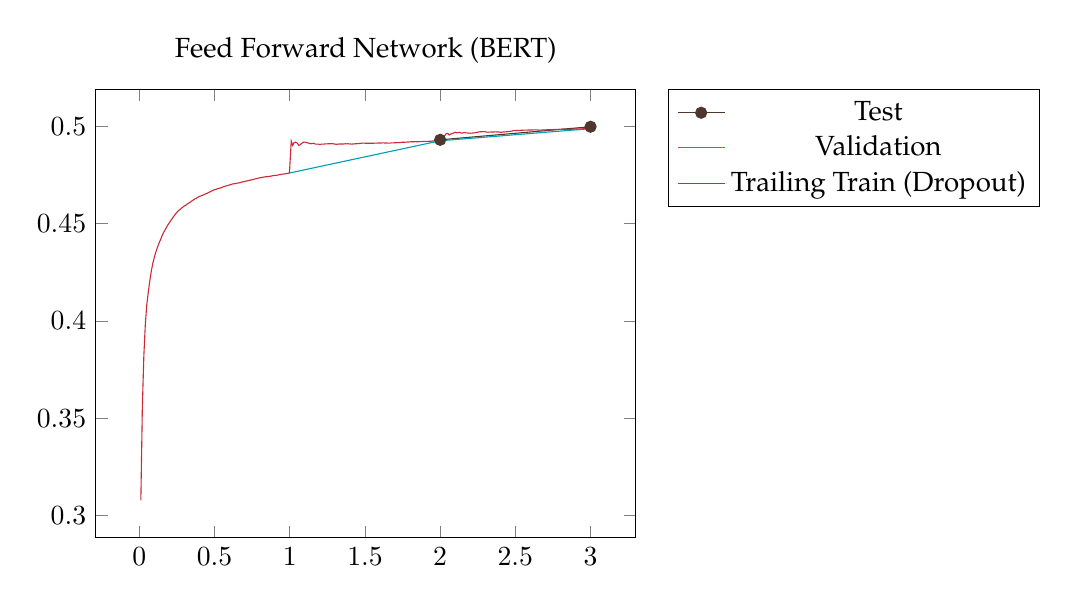
\begin{tikzpicture}
      \begin{axis}[
      title = Feed Forward Network (BERT),
      legend style={at={(1.75,1)},anchor=north east},
      ]
        \legend{Test, Validation, Trailing Train (Dropout)}
        
        % test_ffn_bert
        \addplot[mark=*, color=custom_four] coordinates {(2, 0.49310136986301367) (3, 0.4998191780821918)};
        
        % validation_ffn_bert
        \addplot[mark=none,color=custom_one] coordinates {
            (1, 0.47606704270749395)
            (2, 0.4926156325543916)
            (3, 0.49883674456083804)
        };
        
        % training_ffn_bert_dict
        \addplot[mark=none,color=custom_three] coordinates {
            (0.01, 0.30781895661157027)
            (0.02, 0.35569473140495866)
            (0.03, 0.3822314049586777)
            (0.04, 0.39855856146694213)
            (0.05, 0.40878099173553717)
            (0.06, 0.41502023071625344)
            (0.07, 0.42077737603305787)
            (0.08, 0.42574089617768596)
            (0.09, 0.4297879361799816)
            (0.1, 0.43282218491735536)
            (0.11, 0.43551312453042823)
            (0.12, 0.43771522038567495)
            (0.13, 0.4398367967260013)
            (0.14, 0.44161608987603307)
            (0.15, 0.4435756714876033)
            (0.16, 0.44533872998450413)
            (0.17, 0.4466342063684978)
            (0.18, 0.4480260703627181)
            (0.19, 0.4494566251631144)
            (0.2, 0.45047940340909093)
            (0.21, 0.4517199183392365)
            (0.22, 0.45277428859879787)
            (0.23, 0.4538857572763205)
            (0.24, 0.45493688662190085)
            (0.25, 0.45583677685950413)
            (0.26, 0.4566848279561348)
            (0.27, 0.45725842707376796)
            (0.28, 0.4579501641824085)
            (0.29, 0.4585296291678541)
            (0.3, 0.45917376893939393)
            (0.31, 0.4595711976806185)
            (0.319, 0.4601717862215909)
            (0.32899999999999996, 0.4605931473829201)
            (0.33899999999999997, 0.46111980432668936)
            (0.349, 0.46165049439197164)
            (0.359, 0.46218757174012853)
            (0.369, 0.46274186117936117)
            (0.379, 0.4630783764680296)
            (0.389, 0.4635855385145158)
            (0.39899999999999997, 0.46398502066115704)
            (0.409, 0.4642744658335013)
            (0.419, 0.4645516651908697)
            (0.429, 0.4648948022775322)
            (0.439, 0.4652560926934636)
            (0.449, 0.4656006083562902)
            (0.45899999999999996, 0.4659862895256917)
            (0.469, 0.4663315181554422)
            (0.479, 0.46671347710055094)
            (0.489, 0.4671220115112161)
            (0.499, 0.4674270402892562)
            (0.509, 0.4676441470183115)
            (0.519, 0.4679410610696122)
            (0.529, 0.4681567226726961)
            (0.539, 0.4683590162993572)
            (0.5489999999999999, 0.4686032588279489)
            (0.5589999999999999, 0.46899846424881936)
            (0.569, 0.469216688415253)
            (0.579, 0.46943017063265885)
            (0.589, 0.46968292565485364)
            (0.599, 0.46988959194214874)
            (0.609, 0.4701519314794743)
            (0.619, 0.4703927910890429)
            (0.629, 0.4705250557523285)
            (0.639, 0.4706375500387397)
            (0.649, 0.4708325055626192)
            (0.659, 0.47093448691460055)
            (0.669, 0.47104354261749104)
            (0.679, 0.4713668266893534)
            (0.6890000000000001, 0.4715272787160139)
            (0.6990000000000001, 0.47167207792207794)
            (0.7090000000000001, 0.47184962824467463)
            (0.7190000000000001, 0.4720572199265381)
            (0.7290000000000001, 0.47221092069512055)
            (0.7390000000000001, 0.4724241609895019)
            (0.7490000000000001, 0.47258953168044077)
            (0.759, 0.4727870813397129)
            (0.769, 0.47297782279703765)
            (0.779, 0.47317360669633396)
            (0.789, 0.4733754674913694)
            (0.799, 0.4735109439566116)
            (0.809, 0.47371122844607694)
            (0.8190000000000001, 0.4738034796412014)
            (0.8290000000000001, 0.4739744100368416)
            (0.8390000000000001, 0.47409784226190477)
            (0.8490000000000001, 0.4741268382352941)
            (0.8590000000000001, 0.47426026751393424)
            (0.8690000000000001, 0.474369849553529)
            (0.879, 0.4745139932381668)
            (0.889, 0.47467774979106697)
            (0.899, 0.47478119260789714)
            (0.909, 0.47485220745163925)
            (0.919, 0.47495290884387353)
            (0.929, 0.4751392684173109)
            (0.9390000000000001, 0.4752811373527343)
            (0.948, 0.4754472053066551)
            (0.958, 0.47550220331869836)
            (0.968, 0.4756083193107268)
            (0.978, 0.4757794711376286)
            (0.988, 0.47588292532765675)
            (0.998, 0.4760362861570248)
            (1.01, 0.49247804752066116)
            (1.02, 0.4902182334710744)
            (1.03, 0.49175705922865015)
            (1.04, 0.49184045712809915)
            (1.05, 0.49145144628099174)
            (1.06, 0.49024513601928377)
            (1.07, 0.4906194657615112)
            (1.08, 0.49125936208677684)
            (1.09, 0.4918395603764922)
            (1.1, 0.4919453770661157)
            (1.11, 0.4916973844853494)
            (1.12, 0.4915364583333333)
            (1.13, 0.4913059241894469)
            (1.1400000000000001, 0.4910737345041322)
            (1.15, 0.49122976928374656)
            (1.16, 0.49133603434917356)
            (1.17, 0.49087528864851726)
            (1.18, 0.4908979711891644)
            (1.19, 0.49091656698564595)
            (1.2, 0.4906944085743802)
            (1.21, 0.49089771497441953)
            (1.22, 0.4908682968632607)
            (1.23, 0.49092846074380164)
            (1.24, 0.4910374160640496)
            (1.25, 0.49104855371900824)
            (1.26, 0.491066284567705)
            (1.27, 0.49108270202020204)
            (1.28, 0.4911348417207792)
            (1.29, 0.4910598193929895)
            (1.3, 0.49089940599173554)
            (1.31, 0.4907743351772861)
            (1.319, 0.4908608680914256)
            (1.329, 0.49097150482093666)
            (1.339, 0.4909616933033544)
            (1.349, 0.4909699675324675)
            (1.359, 0.49095446654040403)
            (1.369, 0.4910890035179808)
            (1.379, 0.4910329559047412)
            (1.389, 0.4910766317016317)
            (1.399, 0.49098414901859505)
            (1.409, 0.4909024768191897)
            (1.419, 0.4909522887150728)
            (1.429, 0.490999033009802)
            (1.439, 0.49108327268031554)
            (1.449, 0.4911185720844812)
            (1.459, 0.4912133938196191)
            (1.4689999999999999, 0.49123755385088796)
            (1.479, 0.4913710076618457)
            (1.4889999999999999, 0.4914133654494856)
            (1.499, 0.4913675103305785)
            (1.509, 0.49131079342894185)
            (1.5190000000000001, 0.49133758641926256)
            (1.529, 0.49134935872446595)
            (1.5390000000000001, 0.4913493361646771)
            (1.549, 0.49133170548459804)
            (1.559, 0.49135851719303425)
            (1.569, 0.49139005183413076)
            (1.579, 0.4914199424693645)
            (1.589, 0.4914542915674464)
            (1.599, 0.4914487560261708)
            (1.609, 0.4914672173485978)
            (1.619, 0.49153194564782726)
            (1.629, 0.49148342188114913)
            (1.639, 0.4914646621577996)
            (1.649, 0.49144399634456454)
            (1.659, 0.4914029238667668)
            (1.669, 0.4914204159985198)
            (1.679, 0.4915584551227516)
            (1.689, 0.49156008578871724)
            (1.699, 0.491573199527745)
            (1.709, 0.49161413470492377)
            (1.719, 0.4916606584308999)
            (1.729, 0.49168291138344844)
            (1.739, 0.4917870155796292)
            (1.749, 0.4918358298898072)
            (1.759, 0.4918578729882558)
            (1.7690000000000001, 0.491875150933777)
            (1.779, 0.49194744649290106)
            (1.7890000000000001, 0.49198808060466576)
            (1.799, 0.4920309271694215)
            (1.8090000000000002, 0.4921205425466789)
            (1.819, 0.49210206800544243)
            (1.8290000000000002, 0.492123711789306)
            (1.839, 0.49214868346615503)
            (1.8490000000000002, 0.4920990064414195)
            (1.859, 0.49214808463867)
            (1.8690000000000002, 0.4921385188087774)
            (1.879, 0.4921941033527423)
            (1.889, 0.4922654871622249)
            (1.899, 0.49229044708448116)
            (1.909, 0.49229108959222595)
            (1.919, 0.4923145268145886)
            (1.929, 0.4923752971429841)
            (1.939, 0.4923698649331809)
            (1.948, 0.4924630953675511)
            (1.958, 0.4924881359762397)
            (1.968, 0.4924870335264548)
            (1.978, 0.4925485431776016)
            (1.988, 0.49254620064279153)
            (1.998, 0.49259555785123965)
            (2.01, 0.49548037190082644)
            (2.02, 0.49359181301652894)
            (2.03, 0.4951683023415978)
            (2.04, 0.4962309529958678)
            (2.05, 0.49639721074380166)
            (2.06, 0.4955879820936639)
            (2.07, 0.49605685507674147)
            (2.08, 0.49637622675619836)
            (2.09, 0.49661745293847565)
            (2.1, 0.49700090392561985)
            (2.11, 0.4967423459804658)
            (2.12, 0.49677976497933884)
            (2.13, 0.49696290924984104)
            (2.14, 0.49653879501180637)
            (2.15, 0.4966102789256198)
            (2.16, 0.49685240185950413)
            (2.17, 0.4966501579970831)
            (2.18, 0.4966497359963269)
            (2.19, 0.49655590745976513)
            (2.2, 0.4964892174586777)
            (2.21, 0.49656108569460844)
            (2.22, 0.4965926699849737)
            (2.23, 0.49668747754222065)
            (2.24, 0.4968927556818182)
            (2.25, 0.49700154958677684)
            (2.26, 0.4972112404640814)
            (2.27, 0.4972392007193144)
            (2.2800000000000002, 0.49728245830873674)
            (2.29, 0.49732607224280423)
            (2.3, 0.4972354941460055)
            (2.31, 0.49704037256731537)
            (2.319, 0.4970128083032025)
            (2.3289999999999997, 0.49703974142248936)
            (2.339, 0.49711921183762764)
            (2.349, 0.4971129722550177)
            (2.359, 0.49710618256427913)
            (2.3689999999999998, 0.49718875642171095)
            (2.379, 0.4971047194432362)
            (2.3890000000000002, 0.49713839664123755)
            (2.399, 0.49700009684917357)
            (2.409, 0.4970094864946583)
            (2.419, 0.4971344942935852)
            (2.429, 0.49714482630213336)
            (2.439, 0.4972295266716754)
            (2.449, 0.49733987603305785)
            (2.459, 0.49742577703916635)
            (2.469, 0.4974791739933181)
            (2.479, 0.49760231039084024)
            (2.489, 0.49783044674481364)
            (2.499, 0.4978783574380165)
            (2.509, 0.4978775471965646)
            (2.519, 0.49792643436109346)
            (2.529, 0.49797408584125996)
            (2.539, 0.4980002439164371)
            (2.549, 0.4980060809541698)
            (2.559, 0.4980970290363046)
            (2.569, 0.4981151225170364)
            (2.5789999999999997, 0.49809975242234256)
            (2.589, 0.498146186440678)
            (2.599, 0.49814372417355374)
            (2.609, 0.49814504724969516)
            (2.6189999999999998, 0.49822911806851505)
            (2.629, 0.4981977854847173)
            (2.6390000000000002, 0.49817802492252067)
            (2.649, 0.49817277892561984)
            (2.659, 0.49806595135236664)
            (2.669, 0.4980572344887135)
            (2.6790000000000003, 0.49819879527224115)
            (2.689, 0.49824735746796023)
            (2.699, 0.49821336334120425)
            (2.709, 0.4982544414212548)
            (2.7190000000000003, 0.49830379433539945)
            (2.729, 0.4982894401675535)
            (2.739, 0.49837101435112796)
            (2.749, 0.4983630337465565)
            (2.759, 0.4984219531589822)
            (2.769, 0.4984189686862724)
            (2.779, 0.4984673825227802)
            (2.789, 0.4984561342713673)
            (2.799, 0.49843911415289255)
            (2.809, 0.4985197620140802)
            (2.819, 0.49854293174259223)
            (2.829, 0.49851731305386837)
            (2.839, 0.4985242030696576)
            (2.849, 0.49844281720952843)
            (2.859, 0.49846505321449164)
            (2.869, 0.49852017431366963)
            (2.879, 0.49857807804282495)
            (2.8890000000000002, 0.49863250417866095)
            (2.899, 0.49866455750688704)
            (2.909, 0.49868561835891384)
            (2.919, 0.49871359032518864)
            (2.9290000000000003, 0.4987517217630854)
            (2.939, 0.49873031420344643)
            (2.948, 0.49877120487168336)
            (2.958, 0.49876988098312675)
            (2.968, 0.49877424224674105)
            (2.9779999999999998, 0.4988219978073874)
            (2.988, 0.49880357031054345)
            (2.998, 0.49882747933884297)
        };
     
      \end{axis}
    \end{tikzpicture}
	\caption{Feed Forward Network (BERT)}
	\label{fig:ffn_bert_results}
\end{figure}

% lstm_w2v
\begin{figure}[hbt]
	\center
	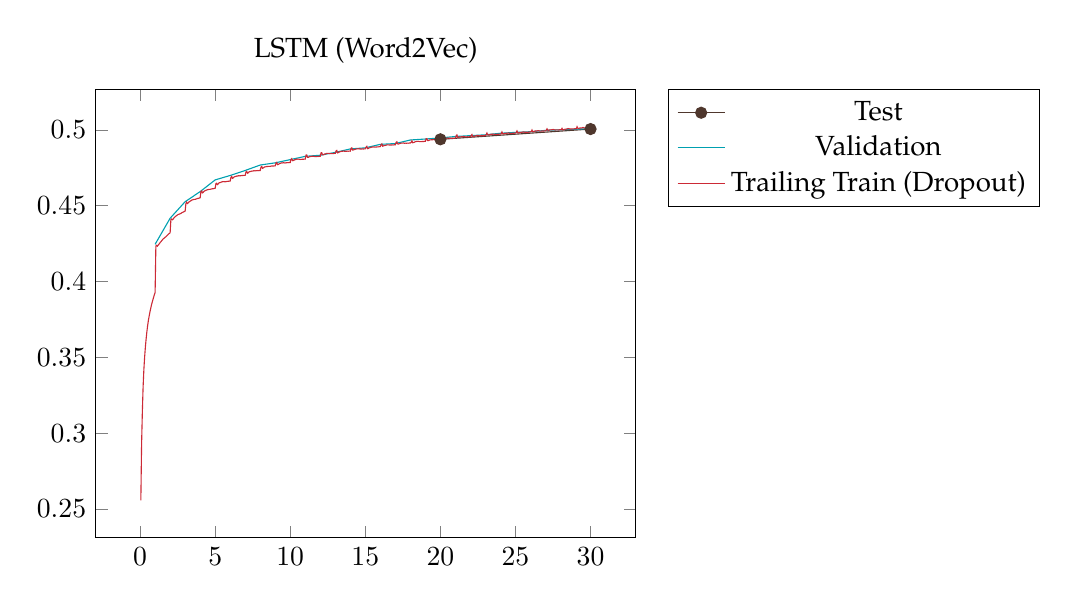
\begin{tikzpicture}
      \begin{axis}[
      title = LSTM (Word2Vec),
      legend style={at={(1.75,1)},anchor=north east},
      ]
        \legend{Test, Validation, Trailing Train (Dropout)}
        
        % test_lstm_w2v
        \addplot[mark=*, color=custom_four] coordinates {(20, 0.4937260273972603) (30, 0.5004931506849315)};
        
        % validation_lstm_w2v
        \addplot[mark=none,color=custom_one] coordinates {
            (1, 0.4245205479452055)
            (2, 0.4416904109589041)
            (3, 0.4526054794520548)
            (4, 0.4592383561643836)
            (5, 0.46696712328767126)
            (6, 0.4698986301369863)
            (7, 0.4731917808219178)
            (8, 0.4767780821917808)
            (9, 0.47822191780821915)
            (10, 0.48034246575342465)
            (11, 0.4825013698630137)
            (12, 0.48323013698630135)
            (13, 0.4851095890410959)
            (14, 0.48738904109589043)
            (15, 0.4881150684931507)
            (16, 0.4904109589041096)
            (17, 0.49093424657534246)
            (18, 0.4932931506849315)
            (19, 0.49392054794520546)
            (20, 0.49463013698630137)
            (21, 0.4956054794520548)
            (22, 0.4961506849315068)
            (23, 0.4967068493150685)
            (24, 0.49772328767123286)
            (25, 0.4983123287671233)
            (26, 0.49874794520547944)
            (27, 0.499613698630137)
            (28, 0.5000520547945205)
            (29, 0.5003671232876712)
            (30, 0.5008164383561644)
        };
        
        % training_lstm_w2v_dict
        \addplot[mark=none,color=custom_three] coordinates {
            (0.05, 0.2556853341584158)
            (0.1, 0.29287850660066006)
            (0.15, 0.31389877268976896)
            (0.2, 0.3303625528568482)
            (0.25, 0.3416544193481848)
            (0.3, 0.3498693619361936)
            (0.35, 0.35648260696605377)
            (0.4, 0.36195539719987624)
            (0.45, 0.36672553974147415)
            (0.5, 0.370730198019802)
            (0.55, 0.37418575841959195)
            (0.6, 0.37700200684130913)
            (0.65, 0.37960638010916475)
            (0.7, 0.3819335477074493)
            (0.75, 0.3841577712458746)
            (0.8, 0.386091679236283)
            (0.85, 0.38785797812317996)
            (0.9, 0.38960134620232856)
            (0.95, 0.39119597609431994)
            (1.0, 0.3926430680177393)
            (1.05, 0.42340591481023104)
            (1.1, 0.4238522973391089)
            (1.15, 0.4233145970847085)
            (1.2, 0.4238788869121287)
            (1.25, 0.4245275113448845)
            (1.3, 0.4251538435093509)
            (1.35, 0.4258125589344649)
            (1.4, 0.42640167337046203)
            (1.45, 0.42702711026310963)
            (1.5, 0.427605133560231)
            (1.55, 0.4281861779927993)
            (1.6, 0.4285377024030528)
            (1.65, 0.42898141977659304)
            (1.7, 0.42933159108321545)
            (1.75, 0.4297998745187019)
            (1.8, 0.4303192037953795)
            (1.85, 0.43075677052999417)
            (1.9, 0.4312689081408141)
            (1.95, 0.43172391355089457)
            (2.0, 0.4320870075288779)
            (2.05, 0.4407648772689769)
            (2.1, 0.4411999793729373)
            (2.15, 0.44065207301980197)
            (2.2, 0.44111215320750824)
            (2.25, 0.44188002784653463)
            (2.3, 0.4423656232810781)
            (2.35, 0.44284415885785006)
            (2.4, 0.4431901686262376)
            (2.45, 0.44357388212779614)
            (2.5, 0.443954336839934)
            (2.55, 0.4442055533678368)
            (2.6, 0.4443552753712871)
            (2.65, 0.444560306391216)
            (2.7, 0.44481224768682226)
            (2.75, 0.445094196919692)
            (2.8, 0.4454383975995256)
            (2.85, 0.44567499029314694)
            (2.9, 0.4459191361844518)
            (2.95, 0.44616845525013027)
            (3.0, 0.4463494933477723)
            (3.05, 0.45139748349834985)
            (3.1, 0.4523079749381188)
            (3.15, 0.45141682136963696)
            (3.2, 0.4517512053939769)
            (3.25, 0.45240047442244224)
            (3.3, 0.4527312594540704)
            (3.35, 0.4530287710690712)
            (3.4, 0.45333247924401815)
            (3.45, 0.45370155505133847)
            (3.5, 0.4538259978341584)
            (3.55, 0.4539776243249325)
            (3.6, 0.454124123349835)
            (3.65, 0.4541104876713633)
            (3.7, 0.45424061100306456)
            (3.75, 0.45443245496424645)
            (3.8, 0.454673439756085)
            (3.85, 0.45473174959959234)
            (3.9, 0.4548700638292996)
            (3.95, 0.455025539560535)
            (4.0, 0.45511212742367985)
            (4.05, 0.4593356796617162)
            (4.1, 0.45972404857673266)
            (4.15, 0.45842250240649063)
            (4.2, 0.45872331373762376)
            (4.25, 0.45936017429867987)
            (4.3, 0.45973318034928495)
            (4.35, 0.4599167366513437)
            (4.4, 0.4601349783415842)
            (4.45, 0.46043543156398975)
            (4.5, 0.4604585653877888)
            (4.55, 0.4606653048117312)
            (4.6, 0.4606826161131738)
            (4.65, 0.4607027184088601)
            (4.7, 0.4608573859618105)
            (4.75, 0.46096092031078106)
            (4.8, 0.46111295089469884)
            (4.85, 0.4611174180377597)
            (4.9, 0.46124171336404474)
            (4.95, 0.46135869240706967)
            (5.0, 0.461403220400165)
            (5.05, 0.4645053372524752)
            (5.1, 0.46478251340759075)
            (5.15, 0.46387470778327833)
            (5.2, 0.46426361386138615)
            (5.25, 0.46495204207920793)
            (5.3, 0.465154767429868)
            (5.35, 0.46526780189179634)
            (5.4, 0.4654653819874175)
            (5.45, 0.46571610286028603)
            (5.5, 0.46571524339933995)
            (5.55, 0.46584638932643263)
            (5.6, 0.46581520945063254)
            (5.65, 0.46572684612211224)
            (5.7, 0.46579706101190477)
            (5.75, 0.46587338421342134)
            (5.8, 0.4660348420095916)
            (5.85, 0.4660421292588818)
            (5.9, 0.4660887149912908)
            (5.95, 0.46615075261638006)
            (6.0, 0.46621029290429045)
            (6.05, 0.46862430383663367)
            (6.1, 0.4692576191212871)
            (6.15, 0.4680366474147415)
            (6.2, 0.4682488268358086)
            (6.25, 0.46885313531353134)
            (6.3, 0.46911795671754675)
            (6.35, 0.46921134635785006)
            (6.4, 0.4693373878403465)
            (6.45, 0.4695775892693436)
            (6.5, 0.46950159859735974)
            (6.55, 0.46974209139663964)
            (6.6, 0.46972038512444997)
            (6.65, 0.4696440046648896)
            (6.7, 0.46972426037246584)
            (6.75, 0.46979252612761274)
            (6.8, 0.46988569706580036)
            (6.85, 0.46986022131624927)
            (6.9, 0.4699423230083425)
            (6.95, 0.46998372226202884)
            (7.0, 0.4700018048679868)
            (7.05, 0.47223726278877887)
            (7.1, 0.4726272431930693)
            (7.15, 0.47135309234048406)
            (7.2, 0.4715999187809406)
            (7.25, 0.47222437087458746)
            (7.3, 0.4724553510038504)
            (7.35, 0.47251674107142855)
            (7.4, 0.4726348977671205)
            (7.45, 0.47282635164558123)
            (7.5, 0.47274617110148515)
            (7.55, 0.4729662419366937)
            (7.6, 0.47300997189562705)
            (7.65, 0.47292078216235084)
            (7.7, 0.47298591466289486)
            (7.75, 0.4730644939493949)
            (7.8, 0.4731366752397896)
            (7.85, 0.4730282196418171)
            (7.9, 0.4731092575403374)
            (7.95, 0.47319194296074346)
            (8.0, 0.4731912644389439)
            (8.05, 0.47536032900165015)
            (8.1, 0.47587761705858084)
            (8.15, 0.47462441556655666)
            (8.2, 0.47482531456270627)
            (8.25, 0.475190800330033)
            (8.3, 0.47558862331545654)
            (8.35, 0.4755758081388496)
            (8.4, 0.4757233169606023)
            (8.45, 0.4758376879354602)
            (8.5, 0.4757741594471947)
            (8.55, 0.47592464324557454)
            (8.6, 0.47587224542766776)
            (8.65, 0.4758603865194212)
            (8.7, 0.47599249322253656)
            (8.75, 0.47609409378437845)
            (8.8, 0.47617836124432755)
            (8.85, 0.4761220894607843)
            (8.9, 0.47615676281169783)
            (8.95, 0.4761815100095536)
            (9.0, 0.4761784821060231)
            (9.05, 0.4780321782178218)
            (9.1, 0.47845599989686466)
            (9.15, 0.47702446025852585)
            (9.2, 0.47714263613861385)
            (9.25, 0.47747202454620463)
            (9.3, 0.47787210361661164)
            (9.35, 0.47788990673620935)
            (9.4, 0.47806843672648514)
            (9.45, 0.4782395231710671)
            (9.5, 0.47813305744636964)
            (9.55, 0.47829499746849685)
            (9.6, 0.4782287799092409)
            (9.65, 0.47810952970297027)
            (9.7, 0.47821220459099484)
            (9.75, 0.478288297579758)
            (9.8, 0.4783705909653465)
            (9.85, 0.47830499387254904)
            (9.9, 0.47838419909699303)
            (9.95, 0.47844539799374675)
            (10.0, 0.4784455252165842)
            (10.05, 0.480491310849835)
            (10.1, 0.4809860380569307)
            (10.15, 0.4796447418179318)
            (10.2, 0.4797451913160066)
            (10.25, 0.4799775680693069)
            (10.3, 0.48027322263476346)
            (10.35, 0.48033016192244227)
            (10.4, 0.4805827628661304)
            (10.45, 0.48071799367436746)
            (10.5, 0.4806108833539604)
            (10.55, 0.4806697466621662)
            (10.6, 0.4805420727619637)
            (10.65, 0.4804332972359736)
            (10.7, 0.48048417425447904)
            (10.75, 0.4805072108773377)
            (10.8, 0.4805952519080033)
            (10.85, 0.4805339679188507)
            (10.9, 0.4806017873922809)
            (10.95, 0.480688082171704)
            (11.0, 0.4806816277330858)
            (11.05, 0.48335331580033003)
            (11.1, 0.48338393409653463)
            (11.15, 0.48186107673267325)
            (11.2, 0.48181756652227725)
            (11.25, 0.4820783054867987)
            (11.3, 0.4823294829482948)
            (11.35, 0.4822901933050448)
            (11.4, 0.4824863345709571)
            (11.45, 0.4825497198157316)
            (11.5, 0.48252114273927393)
            (11.55, 0.4825903488786379)
            (11.6, 0.48246081932411994)
            (11.65, 0.4823479944148261)
            (11.7, 0.4823749115983027)
            (11.75, 0.48239974388063805)
            (11.8, 0.4824808957946576)
            (11.85, 0.48240158919384585)
            (11.9, 0.4824616250687569)
            (11.95, 0.48255622231631057)
            (12.0, 0.48256062422648516)
            (12.05, 0.4848101021039604)
            (12.1, 0.48491323741749176)
            (12.15, 0.4834929782040704)
            (12.2, 0.4835047957920792)
            (12.25, 0.48380388820132014)
            (12.3, 0.4840994353341584)
            (12.35, 0.4840706587399811)
            (12.4, 0.4843472018100248)
            (12.45, 0.48445987176842686)
            (12.5, 0.4844239892739274)
            (12.55, 0.48448897624137416)
            (12.6, 0.48433874149133666)
            (12.65, 0.4842507913651942)
            (12.7, 0.48429741830209805)
            (12.75, 0.4843030201457646)
            (12.8, 0.4843369285659035)
            (12.85, 0.4842999235585323)
            (12.9, 0.48438413177255224)
            (12.95, 0.48446778785608824)
            (13.0, 0.48443607544348183)
            (13.05, 0.48609607054455445)
            (13.1, 0.48641836839933994)
            (13.15, 0.4848101021039604)
            (13.2, 0.48495674762788776)
            (13.25, 0.48527227722772276)
            (13.3, 0.4855191573844885)
            (13.35, 0.4856287386551155)
            (13.4, 0.4858108369430693)
            (13.45, 0.4858715363723872)
            (13.5, 0.48589398978960396)
            (13.55, 0.48601198010426044)
            (13.6, 0.4858508555933718)
            (13.65, 0.48580575455382075)
            (13.7, 0.4858437573668081)
            (13.75, 0.48585327282728275)
            (13.8, 0.48593431730868397)
            (13.85, 0.48587254750291203)
            (13.9, 0.4859019756142281)
            (13.95, 0.48595035798810143)
            (14.0, 0.48589463438531355)
            (14.05, 0.4878010261963696)
            (14.1, 0.4881346044760726)
            (14.15, 0.48663753094059403)
            (14.2, 0.486726968595297)
            (14.25, 0.4869488706683168)
            (14.3, 0.4870538323363586)
            (14.35, 0.487254040694248)
            (14.4, 0.4874005711117987)
            (14.45, 0.48742680257609095)
            (14.5, 0.4874581012788779)
            (14.55, 0.4875575448169817)
            (14.6, 0.48741265728135313)
            (14.65, 0.4873267525069815)
            (14.7, 0.48732011175447904)
            (14.75, 0.4873266037541254)
            (14.8, 0.4874164845683787)
            (14.85, 0.4873560655697923)
            (14.9, 0.4873766673542354)
            (14.95, 0.48745905120939725)
            (15.0, 0.487455684044967)
            (15.05, 0.4885648721122112)
            (15.1, 0.4891288933580858)
            (15.15, 0.4875915325907591)
            (15.2, 0.4877309264129538)
            (15.25, 0.48806466584158414)
            (15.3, 0.48823290532178215)
            (15.35, 0.48832913425271096)
            (15.4, 0.48848671488242573)
            (15.45, 0.4886289735744408)
            (15.5, 0.48865930538366337)
            (15.55, 0.48872397005325535)
            (15.6, 0.48863953778190317)
            (15.65, 0.4886000769548109)
            (15.7, 0.48864337466112684)
            (15.75, 0.4886319100660066)
            (15.8, 0.48876832263304454)
            (15.85, 0.48872222930013587)
            (15.9, 0.48879871711129447)
            (15.95, 0.4889068470991836)
            (16.0, 0.48889925613655116)
            (16.05, 0.49027305074257427)
            (16.1, 0.4906807575288779)
            (16.15, 0.4891922786028603)
            (16.2, 0.489369005259901)
            (16.25, 0.4896071833745875)
            (16.3, 0.48965746183993397)
            (16.35, 0.48977302864214994)
            (16.4, 0.4899430983137376)
            (16.45, 0.4900538882013201)
            (16.5, 0.4900848287953795)
            (16.55, 0.49009051295754574)
            (16.6, 0.4899682106882563)
            (16.65, 0.4899460423806804)
            (16.7, 0.4899638750147336)
            (16.75, 0.48998169348184817)
            (16.8, 0.49005006091429454)
            (16.85, 0.4900032684794215)
            (16.9, 0.49007412134442613)
            (16.95, 0.49018806588718083)
            (17.0, 0.4901699154290429)
            (17.05, 0.4917008302392739)
            (17.1, 0.49211176000412543)
            (17.15, 0.49076616646039606)
            (17.2, 0.49056070157797027)
            (17.25, 0.49080161922442245)
            (17.3, 0.49096061949944997)
            (17.35, 0.491064522188826)
            (17.4, 0.4912109375)
            (17.45, 0.49121308615236525)
            (17.5, 0.49126121596534655)
            (17.55, 0.4913058688681368)
            (17.6, 0.49115131239686466)
            (17.65, 0.4911578823146738)
            (17.7, 0.4911998872878359)
            (17.75, 0.4911400319719472)
            (17.8, 0.4912119446807962)
            (17.85, 0.49114401329838864)
            (17.9, 0.4912109375)
            (17.95, 0.4913320536412194)
            (18.0, 0.49128925587871286)
            (18.05, 0.4916814923679868)
            (18.1, 0.49277085911716173)
            (18.15, 0.4914934852860286)
            (18.2, 0.49157110535272275)
            (18.25, 0.4917388613861386)
            (18.3, 0.4920215166047855)
            (18.35, 0.492215585955917)
            (18.4, 0.49233777137479373)
            (18.45, 0.4923192840117345)
            (18.5, 0.4923612185437294)
            (18.55, 0.4923665218084308)
            (18.6, 0.49224631935849833)
            (18.65, 0.4921971689356436)
            (18.7, 0.4921953272336162)
            (18.75, 0.4922259608773377)
            (18.8, 0.49231521052495875)
            (18.85, 0.49227205579013783)
            (18.9, 0.492332892143381)
            (18.95, 0.49246535467691505)
            (19.0, 0.49245275113448844)
            (19.05, 0.4940761654290429)
            (19.1, 0.4941519054249175)
            (19.15, 0.4928396159928493)
            (19.2, 0.49286351975041254)
            (19.25, 0.4931311881188119)
            (19.3, 0.4933681844746975)
            (19.35, 0.4933643475954738)
            (19.4, 0.4934589650371287)
            (19.45, 0.4934193940227356)
            (19.5, 0.4934937732054455)
            (19.55, 0.4935587308730873)
            (19.6, 0.4934243180177393)
            (19.65, 0.4934580973121351)
            (19.7, 0.4934739288661009)
            (19.75, 0.493441023789879)
            (19.8, 0.4935153671617162)
            (19.85, 0.49345962859153564)
            (19.9, 0.49349495496424645)
            (19.95, 0.4936110387354525)
            (20.0, 0.49359175175330033)
            (20.05, 0.4943694564768977)
            (20.1, 0.49510268409653463)
            (20.15, 0.49388600969471946)
            (20.2, 0.4939673899030528)
            (20.25, 0.4941464263613861)
            (20.3, 0.4943017739273927)
            (20.35, 0.494413657325554)
            (20.4, 0.49447863487520627)
            (20.45, 0.494472591790429)
            (20.5, 0.49454865408415843)
            (20.55, 0.49457250412541254)
            (20.6, 0.4944468079620462)
            (20.65, 0.49440813221947194)
            (20.7, 0.4944401317921971)
            (20.75, 0.4944274700907591)
            (20.8, 0.49448991530012376)
            (20.85, 0.49439808410988156)
            (20.9, 0.49445235864732306)
            (20.95, 0.49453840840498525)
            (21.0, 0.49451255672442246)
            (21.05, 0.49605507425742573)
            (21.1, 0.49663843337458746)
            (21.15, 0.49503016707920794)
            (21.2, 0.4950196923989274)
            (21.25, 0.4952435282590759)
            (21.3, 0.4953175493330583)
            (21.35, 0.49534417727487035)
            (21.4, 0.49541611876031355)
            (21.45, 0.49545273537770446)
            (21.5, 0.4955387530940594)
            (21.55, 0.495551410609811)
            (21.6, 0.4954311593268702)
            (21.65, 0.4953670922981721)
            (21.7, 0.4953695006777463)
            (21.75, 0.4953458041116612)
            (21.8, 0.49540342828228134)
            (21.85, 0.49529615760289264)
            (21.9, 0.4953546135863586)
            (21.95, 0.4954576358129234)
            (22.0, 0.49542433735561053)
            (22.05, 0.4962452299917492)
            (22.1, 0.4968833797442244)
            (22.15, 0.49553724903740376)
            (22.2, 0.4955208655631188)
            (22.25, 0.49567734117161716)
            (22.3, 0.4959186348322332)
            (22.35, 0.4959800248998114)
            (22.4, 0.49606796617161714)
            (22.45, 0.4961062838054639)
            (22.5, 0.49623459416254123)
            (22.55, 0.49619131835058505)
            (22.6, 0.4960174728410341)
            (22.65, 0.4960049941292206)
            (22.7, 0.49610203765912303)
            (22.75, 0.4961019148789879)
            (22.8, 0.49615397941161304)
            (22.85, 0.49604824912638323)
            (22.9, 0.4961415575151265)
            (22.95, 0.4962511670574952)
            (23.0, 0.4962028478238449)
            (23.05, 0.4968414810231023)
            (23.1, 0.4978422158622112)
            (23.15, 0.49662554146039606)
            (23.2, 0.49662070699257427)
            (23.25, 0.496715784859736)
            (23.3, 0.49692581562843785)
            (23.35, 0.4969482997406884)
            (23.4, 0.4970550033518977)
            (23.45, 0.4970541976072607)
            (23.5, 0.4971972978547855)
            (23.55, 0.4971716898252325)
            (23.6, 0.4970045100213146)
            (23.65, 0.4969567644865448)
            (23.7, 0.4970005580357143)
            (23.75, 0.49703142189218924)
            (23.8, 0.49711764999742164)
            (23.85, 0.4970162802125801)
            (23.9, 0.4970769375114595)
            (23.95, 0.49716818926958484)
            (24.0, 0.49712993760313534)
            (24.05, 0.4973700495049505)
            (24.1, 0.49858027794966997)
            (24.15, 0.49737112383113313)
            (24.2, 0.49734668291047857)
            (24.25, 0.4975253970709571)
            (24.3, 0.4976644148789879)
            (24.35, 0.49766840523338046)
            (24.4, 0.4977487494843234)
            (24.45, 0.49773496229831315)
            (24.5, 0.497869611179868)
            (24.55, 0.49786023524227424)
            (24.6, 0.49768079835327284)
            (24.65, 0.4976335899815943)
            (24.7, 0.497664261403819)
            (24.75, 0.49767945544554454)
            (24.8, 0.49776768448329206)
            (24.85, 0.49765727376965635)
            (24.9, 0.4977197426773927)
            (24.95, 0.4978002323258642)
            (25.0, 0.4977735664191419)
            (25.05, 0.4983466120049505)
            (25.1, 0.4992941676980198)
            (25.15, 0.49802216549779976)
            (25.2, 0.4979098984117162)
            (25.25, 0.49814163056930694)
            (25.3, 0.498321365339659)
            (25.35, 0.49822367839462517)
            (25.4, 0.4983671584931931)
            (25.45, 0.49840176074899156)
            (25.5, 0.498575765779703)
            (25.55, 0.4985646025540054)
            (25.6, 0.4983938823569857)
            (25.65, 0.4983649581905306)
            (25.7, 0.49840946008663367)
            (25.75, 0.4983812053080308)
            (25.8, 0.49842617928785066)
            (25.85, 0.4983974213138226)
            (25.9, 0.4984871696805097)
            (25.95, 0.4985808716562446)
            (26.0, 0.49860219420379537)
            (26.05, 0.4988526196369637)
            (26.1, 0.4998710808580858)
            (26.15, 0.49878493708745875)
            (26.2, 0.49875351304661714)
            (26.25, 0.49893126031353136)
            (26.3, 0.4992345425948845)
            (26.35, 0.49918090302333806)
            (26.4, 0.499223262169967)
            (26.45, 0.49924761356343966)
            (26.5, 0.49945112675330033)
            (26.55, 0.49940521395889587)
            (26.6, 0.4991794833780253)
            (26.65, 0.49914144809913685)
            (26.7, 0.4991601838755304)
            (26.75, 0.49919704861111114)
            (26.8, 0.4992669738165223)
            (26.85, 0.4992003221461852)
            (26.9, 0.499269100087092)
            (26.95, 0.4993372538322911)
            (27.0, 0.4993280089727723)
            (27.05, 0.49972604682343236)
            (27.1, 0.5006574876237624)
            (27.15, 0.4998259591584158)
            (27.2, 0.49966400448638615)
            (27.25, 0.4998046875)
            (27.3, 0.5000075202832783)
            (27.35, 0.4999396842586044)
            (27.4, 0.5000016114892739)
            (27.45, 0.5000236351760176)
            (27.5, 0.5002185179455445)
            (27.55, 0.5001312631263126)
            (27.6, 0.4999572955342409)
            (27.65, 0.49988446861513075)
            (27.7, 0.4999304757484677)
            (27.75, 0.4999237228410341)
            (27.8, 0.4999850937242162)
            (27.85, 0.49989743344738885)
            (27.9, 0.49996723305143015)
            (27.95, 0.5000334171986277)
            (28.0, 0.5000325520833333)
            (28.05, 0.5000773514851485)
            (28.1, 0.5009427212252475)
            (28.15, 0.4999290944719472)
            (28.2, 0.49992426000412543)
            (28.25, 0.5001463232260726)
            (28.3, 0.5003948148721122)
            (28.35, 0.500450296145686)
            (28.4, 0.5005080219936056)
            (28.45, 0.500568318550605)
            (28.5, 0.5008254048061056)
            (28.55, 0.5007664828982898)
            (28.6, 0.5005820162094334)
            (28.65, 0.5004995616749175)
            (28.7, 0.5005000221004243)
            (28.75, 0.500518684680968)
            (28.8, 0.5005777189047029)
            (28.85, 0.5005589023975927)
            (28.9, 0.5006222139140998)
            (28.95, 0.5006920922355393)
            (29.0, 0.500701642429868)
            (29.05, 0.5007026093234324)
            (29.1, 0.5020175845709571)
            (29.15, 0.5010592856160616)
            (29.2, 0.5008814846328383)
            (29.25, 0.500990099009901)
            (29.3, 0.5012408467409241)
            (29.35, 0.5011538263201321)
            (29.4, 0.5012186887634076)
            (29.45, 0.5013017252246058)
            (29.5, 0.5015428398308581)
            (29.55, 0.5014034606585659)
            (29.6, 0.5012021709983498)
            (29.65, 0.5011176297918253)
            (29.7, 0.5011839841908298)
            (29.75, 0.5012139885863587)
            (29.8, 0.5012678391862624)
            (29.85, 0.5012717494175888)
            (29.9, 0.501343623945728)
            (29.95, 0.5014097986690116)
            (30.0, 0.5013794348184818)
        };
      
      \end{axis}
    \end{tikzpicture}
	\caption{LSTM (Word2Vec)}
	\label{fig:lstm_w2v_results}
\end{figure}

% lstm_bert
\begin{figure}[hbt]
	\center
	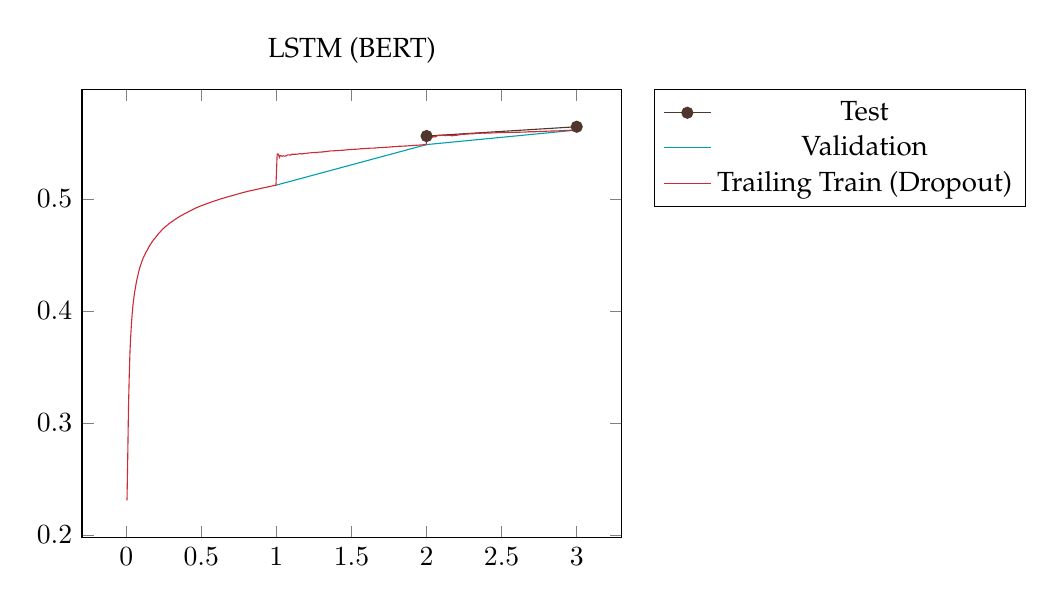
\begin{tikzpicture}
      \begin{axis}[
      title = LSTM (BERT),
      legend style={at={(1.75,1)},anchor=north east},
      ]
        \legend{Test, Validation, Trailing Train (Dropout)}
        
        % test_lstm_bert
        \addplot[mark=*, color=custom_four] coordinates {(2, 0.556) (3, 0.5643123287671233)};
        
        % validation_lstm_bert
        \addplot[mark=none,color=custom_one] coordinates {
            (1, 0.5122243352135375)
            (2, 0.5483864625302176)
            (3, 0.5613624496373892)
        };
        
        % training_lstm_bert_dict
        \addplot[mark=none,color=custom_three] coordinates {
            (0.005, 0.2307889344262295)
            (0.01, 0.27052382172131145)
            (0.015, 0.31452783469945356)
            (0.02, 0.34254930840163933)
            (0.025, 0.3640753073770492)
            (0.03, 0.3781164617486339)
            (0.035, 0.3892893735362998)
            (0.04, 0.39826139856557374)
            (0.045, 0.405609631147541)
            (0.05, 0.4109182889344262)
            (0.055, 0.4158962835320417)
            (0.06, 0.4197777920081967)
            (0.065, 0.42378625472887765)
            (0.07, 0.4273318574355972)
            (0.076, 0.4308785860655738)
            (0.081, 0.4336417776639344)
            (0.086, 0.43661101735776275)
            (0.091, 0.43897284836065575)
            (0.096, 0.44075239969801555)
            (0.10099999999999999, 0.4427414190573771)
            (0.106, 0.4447117730288837)
            (0.111, 0.44641277011922503)
            (0.11599999999999999, 0.4480716544903778)
            (0.121, 0.4493228099385246)
            (0.126, 0.45068391393442625)
            (0.131, 0.4522580390920555)
            (0.136, 0.4532483302975106)
            (0.141, 0.45442860802107726)
            (0.146, 0.45587858606557374)
            (0.151, 0.4570248463114754)
            (0.156, 0.45826860787942886)
            (0.161, 0.4593325755635246)
            (0.166, 0.4602098081222057)
            (0.171, 0.4612689850530376)
            (0.17600000000000002, 0.46230971896955503)
            (0.18100000000000002, 0.46327306750910746)
            (0.18600000000000003, 0.4640649230172796)
            (0.191, 0.46482352782571185)
            (0.196, 0.4655941309373686)
            (0.201, 0.46650230532786885)
            (0.20600000000000002, 0.46735993102758894)
            (0.21100000000000002, 0.4682117852263856)
            (0.21600000000000003, 0.46912379670224935)
            (0.221, 0.4697949655365127)
            (0.22699999999999998, 0.47050887978142075)
            (0.23199999999999998, 0.4714437254989309)
            (0.237, 0.47218346703871644)
            (0.242, 0.4728670380806011)
            (0.247, 0.47344690950150553)
            (0.252, 0.4739856557377049)
            (0.257, 0.47472049783027964)
            (0.262, 0.4752682160308953)
            (0.267, 0.4756816907670894)
            (0.272, 0.47630635245901637)
            (0.27699999999999997, 0.47679769001490313)
            (0.282, 0.47744643771955503)
            (0.287, 0.4780038916450963)
            (0.292, 0.4784968555681176)
            (0.297, 0.47898179181717143)
            (0.302, 0.4794857838114754)
            (0.307, 0.4798462274926095)
            (0.312, 0.4803809574960338)
            (0.317, 0.4809017613192818)
            (0.322, 0.4812401943519467)
            (0.327, 0.48165096941992436)
            (0.332, 0.4821783407848982)
            (0.337, 0.48256285172498165)
            (0.342, 0.4830038572806172)
            (0.34700000000000003, 0.48350818187217864)
            (0.35200000000000004, 0.4838901492974239)
            (0.35700000000000004, 0.4842721802124221)
            (0.36200000000000004, 0.48464893556466304)
            (0.36700000000000005, 0.48510659948349427)
            (0.37200000000000005, 0.48542814715330085)
            (0.37799999999999995, 0.4857889344262295)
            (0.38299999999999995, 0.486219430813201)
            (0.38799999999999996, 0.4865713819991484)
            (0.39299999999999996, 0.4869331914670029)
            (0.39799999999999996, 0.4872761140796846)
            (0.40299999999999997, 0.48760005763319675)
            (0.408, 0.4879191648957701)
            (0.413, 0.488359343762495)
            (0.418, 0.48867781577128183)
            (0.423, 0.48900242730288834)
            (0.428, 0.48933672854387655)
            (0.433, 0.4896781476362943)
            (0.43799999999999994, 0.4900036213962691)
            (0.44299999999999995, 0.4903755472242921)
            (0.44799999999999995, 0.49071896873273163)
            (0.45299999999999996, 0.4910611623406193)
            (0.45799999999999996, 0.4913880944874797)
            (0.46299999999999997, 0.49172532074126873)
            (0.46799999999999997, 0.4920215549532875)
            (0.473, 0.4923005864143704)
            (0.478, 0.4925912694132873)
            (0.483, 0.4929292605874317)
            (0.488, 0.4932259538195031)
            (0.493, 0.49347934614419536)
            (0.498, 0.4937657828282828)
            (0.503, 0.49398821721311476)
            (0.508, 0.49422082961369906)
            (0.513, 0.49445955380102863)
            (0.518, 0.49471042893522205)
            (0.523, 0.4949940396437579)
            (0.529, 0.49520638173302106)
            (0.534, 0.4954678800649551)
            (0.539, 0.49572628600428986)
            (0.544, 0.4959674550318761)
            (0.5489999999999999, 0.4961947990299293)
            (0.5539999999999999, 0.4964779713114754)
            (0.5589999999999999, 0.4967450801211047)
            (0.564, 0.4970308612046253)
            (0.569, 0.49720957855795733)
            (0.574, 0.49741998759706646)
            (0.579, 0.4977058089807555)
            (0.584, 0.4979154889768231)
            (0.589, 0.49810790160431556)
            (0.594, 0.49832038847596555)
            (0.599, 0.4985589010194242)
            (0.604, 0.49875715078551913)
            (0.609, 0.4989727636837827)
            (0.614, 0.49926410071217414)
            (0.619, 0.49947677179128347)
            (0.624, 0.49967774986779484)
            (0.629, 0.4998811475409836)
            (0.634, 0.500059971051262)
            (0.639, 0.5002228685297535)
            (0.644, 0.5004797763511782)
            (0.649, 0.5006527791015377)
            (0.654, 0.5008369128310214)
            (0.659, 0.5010250789951195)
            (0.664, 0.5012526002856433)
            (0.669, 0.5014391447368421)
            (0.674, 0.5016936322485931)
            (0.68, 0.5019201578627808)
            (0.685, 0.5021089794780618)
            (0.69, 0.5022599878844083)
            (0.695, 0.5024510349845569)
            (0.7, 0.5025872744427409)
            (0.705, 0.5027956674473067)
            (0.71, 0.5029933837635159)
            (0.715, 0.5031892172708381)
            (0.72, 0.5033957461595782)
            (0.725, 0.5035607176400273)
            (0.73, 0.5037587443470888)
            (0.735, 0.5039882698461711)
            (0.74, 0.5041702387922382)
            (0.745, 0.5043488833351795)
            (0.75, 0.504575413961932)
            (0.755, 0.5047698941256831)
            (0.76, 0.5049499240039084)
            (0.765, 0.5051225295243744)
            (0.77, 0.5053280362691525)
            (0.775, 0.5054888758782201)
            (0.78, 0.5056757337387625)
            (0.785, 0.50580683191467)
            (0.79, 0.5059676666753681)
            (0.795, 0.5061645634467732)
            (0.8, 0.5063154867769873)
            (0.805, 0.5065201556096312)
            (0.81, 0.5066992127838306)
            (0.815, 0.5068649912720097)
            (0.82, 0.5069564486322036)
            (0.825, 0.5071389412984806)
            (0.831, 0.5073025335320417)
            (0.836, 0.5074433234989136)
            (0.841, 0.507590479900854)
            (0.846, 0.5077263551424668)
            (0.851, 0.5078731266369192)
            (0.856, 0.5080162879701061)
            (0.861, 0.5082000916738568)
            (0.866, 0.5083437827630576)
            (0.871, 0.5084698960011371)
            (0.8759999999999999, 0.5086416672555116)
            (0.8809999999999999, 0.5088133050351288)
            (0.8859999999999999, 0.5089255047270864)
            (0.8909999999999999, 0.5091167540752061)
            (0.8959999999999999, 0.5092824702983975)
            (0.9009999999999999, 0.5094198615944684)
            (0.9059999999999999, 0.5095902350865209)
            (0.9109999999999999, 0.5097116712707183)
            (0.9159999999999999, 0.509838106309674)
            (0.9209999999999999, 0.5099729575382962)
            (0.9259999999999999, 0.5101160877361012)
            (0.9309999999999999, 0.51027013181214)
            (0.9359999999999999, 0.5104022067248369)
            (0.941, 0.5105256777636539)
            (0.946, 0.5107043784879666)
            (0.951, 0.5108422239569781)
            (0.956, 0.5109981665228646)
            (0.961, 0.5111263249935628)
            (0.966, 0.5112834992955942)
            (0.971, 0.5114005563577678)
            (0.976, 0.5115731816165286)
            (0.982, 0.511697732765868)
            (0.987, 0.5118118648586484)
            (0.992, 0.5119485676541566)
            (0.997, 0.5121003839625766)
            (1.005, 0.539702868852459)
            (1.01, 0.5401191086065574)
            (1.015, 0.5388276980874317)
            (1.02, 0.5369652920081968)
            (1.025, 0.5387167008196722)
            (1.03, 0.5383794398907104)
            (1.035, 0.5381842798594848)
            (1.04, 0.5379898821721312)
            (1.045, 0.5384292463570127)
            (1.05, 0.538249231557377)
            (1.055, 0.5381019467213115)
            (1.06, 0.5381926656420765)
            (1.065, 0.5383925756620429)
            (1.07, 0.538847519028103)
            (1.076, 0.5391948428961748)
            (1.081, 0.5392265945184426)
            (1.086, 0.5391077025072324)
            (1.091, 0.5391016336520947)
            (1.096, 0.5390389074633305)
            (1.101, 0.5395876024590164)
            (1.106, 0.5398370413739266)
            (1.111, 0.5397581734351714)
            (1.116, 0.5397418478260869)
            (1.121, 0.539828274419399)
            (1.126, 0.5396900614754099)
            (1.131, 0.5399097572509458)
            (1.1360000000000001, 0.5397645340012144)
            (1.141, 0.5398766832552693)
            (1.146, 0.5400605921424534)
            (1.151, 0.5401319159836065)
            (1.156, 0.5402895293495505)
            (1.161, 0.5403272284836066)
            (1.166, 0.5400017076502732)
            (1.171, 0.540160544238187)
            (1.176, 0.540160275175644)
            (1.181, 0.5403325648907104)
            (1.186, 0.5403795829641117)
            (1.191, 0.5404982743744607)
            (1.196, 0.5404942990752417)
            (1.201, 0.5406009861680328)
            (1.206, 0.540718087764894)
            (1.211, 0.5408052180913349)
            (1.216, 0.5409389296606939)
            (1.221, 0.5409748742548435)
            (1.2269999999999999, 0.54095514571949)
            (1.232, 0.5411548356200998)
            (1.237, 0.5412533789675619)
            (1.242, 0.5412397540983607)
            (1.2469999999999999, 0.5412554366008698)
            (1.252, 0.5412307889344262)
            (1.2570000000000001, 0.5413439709900354)
            (1.262, 0.5413407353404792)
            (1.267, 0.5412796261212496)
            (1.272, 0.5414460951730419)
            (1.277, 0.5415122019374069)
            (1.282, 0.5416411281469555)
            (1.287, 0.5416295926804716)
            (1.292, 0.5416096223148672)
            (1.297, 0.5417303417616004)
            (1.302, 0.5417819330601092)
            (1.307, 0.5417530989653319)
            (1.312, 0.5419018128635642)
            (1.317, 0.5420580031876139)
            (1.322, 0.5420081967213115)
            (1.327, 0.5420879965321563)
            (1.332, 0.542262403750621)
            (1.337, 0.5422911059456814)
            (1.342, 0.5423924180327869)
            (1.347, 0.542552974281302)
            (1.352, 0.5425744657494145)
            (1.357, 0.5426422520780421)
            (1.362, 0.5427632983265027)
            (1.367, 0.5428336584886593)
            (1.372, 0.5427974080638015)
            (1.378, 0.5428005464480874)
            (1.383, 0.5428811205780846)
            (1.388, 0.5428789320310836)
            (1.393, 0.5429309846574191)
            (1.398, 0.542981719495746)
            (1.403, 0.5429887615266393)
            (1.408, 0.5430446455676988)
            (1.413, 0.5431108806477409)
            (1.418, 0.5431469731384555)
            (1.423, 0.5431989778493365)
            (1.428, 0.5432196239151398)
            (1.433, 0.5432628729031643)
            (1.438, 0.5433029194931223)
            (1.443, 0.5433413282414307)
            (1.448, 0.5434364351169645)
            (1.4529999999999998, 0.5435023907103825)
            (1.458, 0.5435929337056387)
            (1.463, 0.5436070306931575)
            (1.468, 0.5436483672659969)
            (1.4729999999999999, 0.543739236353331)
            (1.478, 0.5438187553925798)
            (1.483, 0.5439019541922814)
            (1.488, 0.543930623626838)
            (1.4929999999999999, 0.5439717767229842)
            (1.498, 0.544003042722305)
            (1.5030000000000001, 0.5440157530737705)
            (1.508, 0.5440871763918195)
            (1.513, 0.5440956736178078)
            (1.518, 0.5441686644516951)
            (1.5230000000000001, 0.5442433303121059)
            (1.529, 0.5442281420765027)
            (1.534, 0.5442929844571606)
            (1.5390000000000001, 0.5443213047724835)
            (1.544, 0.5443799332119005)
            (1.549, 0.544443948338096)
            (1.5539999999999998, 0.5445743293591654)
            (1.559, 0.5446158248412347)
            (1.564, 0.5446868825014637)
            (1.569, 0.5446835784491513)
            (1.5739999999999998, 0.5447039248993385)
            (1.579, 0.5448235923022096)
            (1.584, 0.5448490054409271)
            (1.589, 0.5448865726145439)
            (1.5939999999999999, 0.5449386982495138)
            (1.599, 0.544975418446067)
            (1.604, 0.544972037226776)
            (1.609, 0.5449925272659532)
            (1.6139999999999999, 0.5450793427506047)
            (1.619, 0.5451012303411968)
            (1.624, 0.5451661447316235)
            (1.629, 0.545202356557377)
            (1.634, 0.5452430758847254)
            (1.639, 0.5452286973989932)
            (1.6440000000000001, 0.5452710761398566)
            (1.649, 0.5452720922289999)
            (1.654, 0.5453095444514502)
            (1.659, 0.5453493578713553)
            (1.6640000000000001, 0.5454225270119225)
            (1.669, 0.5454594477998275)
            (1.674, 0.5455450399131392)
            (1.6800000000000002, 0.5456397996357013)
            (1.685, 0.545676662698891)
            (1.69, 0.545670919588369)
            (1.6949999999999998, 0.5457000623663578)
            (1.7, 0.5457029867908951)
            (1.705, 0.5457296545667447)
            (1.71, 0.5457854646262063)
            (1.7149999999999999, 0.545847704052182)
            (1.72, 0.5458799653215637)
            (1.725, 0.5459099997153917)
            (1.73, 0.5459599349915206)
            (1.7349999999999999, 0.5460306780541209)
            (1.74, 0.5460551536188246)
            (1.745, 0.546079298432654)
            (1.75, 0.5461529733744086)
            (1.755, 0.5462482923497268)
            (1.76, 0.546282976875475)
            (1.7650000000000001, 0.5463222605694564)
            (1.77, 0.5464221378442087)
            (1.775, 0.5464346424579519)
            (1.78, 0.54647673188789)
            (1.7850000000000001, 0.5465219761454393)
            (1.79, 0.5465380925655215)
            (1.795, 0.5465985876219133)
            (1.8, 0.5466571134910816)
            (1.8050000000000002, 0.5467629354508197)
            (1.81, 0.5468268728999084)
            (1.815, 0.5468765811576604)
            (1.8199999999999998, 0.5468651783918335)
            (1.825, 0.5469089707866853)
            (1.831, 0.5469312748385494)
            (1.8359999999999999, 0.5469641115692278)
            (1.841, 0.5470007730440758)
            (1.846, 0.5470248005708431)
            (1.851, 0.547065216073334)
            (1.8559999999999999, 0.5471134432256509)
            (1.861, 0.5471472503834723)
            (1.866, 0.547155347526687)
            (1.871, 0.5471788975883635)
            (1.876, 0.547246340328811)
            (1.8809999999999998, 0.5473100848946136)
            (1.886, 0.5473512743340164)
            (1.891, 0.5474296245484856)
            (1.896, 0.5474829906520537)
            (1.9009999999999998, 0.5474999856900815)
            (1.906, 0.5475651753187614)
            (1.911, 0.5475932037406032)
            (1.916, 0.5476212760088273)
            (1.9209999999999998, 0.5476577896846726)
            (1.926, 0.5477113078002495)
            (1.931, 0.5477628627603013)
            (1.936, 0.5478221261898466)
            (1.9409999999999998, 0.5478499358946262)
            (1.946, 0.5479070838419952)
            (1.951, 0.5479588835761992)
            (1.956, 0.5480060936151855)
            (1.9609999999999999, 0.5480497918633593)
            (1.966, 0.5481230522114071)
            (1.971, 0.5481301893102862)
            (1.976, 0.5482006295419977)
            (1.982, 0.5482325819672131)
            (1.987, 0.5482312097482436)
            (1.992, 0.54826755845885)
            (1.9969999999999999, 0.5483145362435834)
            (2.005, 0.5594262295081968)
            (2.01, 0.5575051229508197)
            (2.015, 0.5566512978142076)
            (2.02, 0.554383324795082)
            (2.025, 0.555750512295082)
            (2.03, 0.5552104678961749)
            (2.035, 0.5555931645199064)
            (2.04, 0.5550397028688525)
            (2.045, 0.555541325136612)
            (2.05, 0.555251024590164)
            (2.055, 0.5554035488077497)
            (2.06, 0.5553758965163934)
            (2.065, 0.5557859788776797)
            (2.07, 0.5561557742974239)
            (2.076, 0.5565018784153005)
            (2.081, 0.5566286180840164)
            (2.086, 0.5564993671648988)
            (2.091, 0.5565765881147541)
            (2.096, 0.5563726811906816)
            (2.101, 0.5567366803278688)
            (2.106, 0.55682206284153)
            (2.111, 0.5568327356557377)
            (2.116, 0.5567060539914469)
            (2.121, 0.5566512978142076)
            (2.126, 0.5563524590163934)
            (2.1310000000000002, 0.5565987547288777)
            (2.136, 0.5565374544626593)
            (2.141, 0.5567206711065574)
            (2.146, 0.556690308790277)
            (2.151, 0.5566128756830601)
            (2.156, 0.5566168693812797)
            (2.161, 0.5565765881147541)
            (2.166, 0.5561622888723299)
            (2.171, 0.5562507533751205)
            (2.176, 0.556376244145199)
            (2.181, 0.5565410120673953)
            (2.186, 0.5565255316792203)
            (2.191, 0.5566810693485763)
            (2.196, 0.5566545817570407)
            (2.201, 0.5567206711065574)
            (2.206, 0.5568522590963615)
            (2.211, 0.5569836797423887)
            (2.216, 0.557153664696912)
            (2.221, 0.5572096800484352)
            (2.227, 0.5572318989071038)
            (2.232, 0.5574383018531718)
            (2.237, 0.5574737857516567)
            (2.242, 0.5575678257342896)
            (2.247, 0.5575338742054199)
            (2.252, 0.5575076844262296)
            (2.257, 0.5576583092253294)
            (2.262, 0.5577132428278688)
            (2.267, 0.5577201902257964)
            (2.2720000000000002, 0.5577909171979356)
            (2.277, 0.5578159929210134)
            (2.282, 0.5579945477166276)
            (2.287, 0.5579410231521427)
            (2.292, 0.5579235708733747)
            (2.297, 0.5580315278549597)
            (2.302, 0.5580152834699453)
            (2.307, 0.5579019416823434)
            (2.312, 0.5580473707694341)
            (2.317, 0.5581475247202706)
            (2.322, 0.5581504946849385)
            (2.327, 0.5582174101513241)
            (2.332, 0.5583861152508693)
            (2.337, 0.5584312683508686)
            (2.342, 0.5584072896576664)
            (2.347, 0.5584666043003088)
            (2.352, 0.558516905737705)
            (2.357, 0.5585288111867929)
            (2.362, 0.5585217085040983)
            (2.367, 0.5586516463620032)
            (2.372, 0.558586827093487)
            (2.378, 0.5585587431693989)
            (2.383, 0.5585575186044004)
            (2.388, 0.5585213966361507)
            (2.393, 0.5585748673287095)
            (2.398, 0.5586107724631666)
            (2.403, 0.5586321721311476)
            (2.408, 0.5586467187816232)
            (2.413, 0.5586890243902439)
            (2.418, 0.5586971348508789)
            (2.423, 0.5587492681498829)
            (2.428, 0.5587414115236259)
            (2.433, 0.5587888391155166)
            (2.4379999999999997, 0.558792485161108)
            (2.443, 0.5588062360283159)
            (2.448, 0.5588534951188064)
            (2.453, 0.5588669740437159)
            (2.458, 0.5588878974509097)
            (2.463, 0.5589195028510335)
            (2.468, 0.5589662656442799)
            (2.473, 0.5590324707882804)
            (2.4779999999999998, 0.5590541415012942)
            (2.483, 0.5590540151127049)
            (2.488, 0.5590875602078756)
            (2.493, 0.5591374100869856)
            (2.498, 0.5591092792680907)
            (2.503, 0.5590701844262295)
            (2.508, 0.5590908283963643)
            (2.513, 0.5590909775795564)
            (2.518, 0.5591402395352538)
            (2.523, 0.5592039476276797)
            (2.529, 0.5591908177205308)
            (2.534, 0.5592123704763378)
            (2.539, 0.5592173615366938)
            (2.544, 0.5592347117865817)
            (2.549, 0.5592164940216574)
            (2.554, 0.5592713766766021)
            (2.559, 0.5592871944690592)
            (2.564, 0.5593324612119438)
            (2.569, 0.5592941888510082)
            (2.574, 0.5592784952904803)
            (2.5789999999999997, 0.5593248841767641)
            (2.584, 0.5593439752331826)
            (2.589, 0.5593506988230349)
            (2.594, 0.5593746743887191)
            (2.599, 0.559379412625706)
            (2.604, 0.5593531207308743)
            (2.609, 0.5593648387752337)
            (2.614, 0.5594414513907552)
            (2.6189999999999998, 0.5594048838797814)
            (2.624, 0.5594422387295082)
            (2.629, 0.5594743852459017)
            (2.634, 0.5594994145199064)
            (2.6390000000000002, 0.5594978298050859)
            (2.644, 0.559508777055584)
            (2.649, 0.559511612021858)
            (2.654, 0.5595454366330391)
            (2.659, 0.5595792336691278)
            (2.664, 0.5596348345131644)
            (2.669, 0.5596948955380254)
            (2.674, 0.5597626620993393)
            (2.68, 0.5598080790831815)
            (2.685, 0.5598471778567985)
            (2.69, 0.5598305499880339)
            (2.695, 0.5598429332976954)
            (2.7, 0.5598058438495106)
            (2.705, 0.5597930693793911)
            (2.71, 0.5598068175212184)
            (2.715, 0.5598650174613253)
            (2.7199999999999998, 0.5598852351541901)
            (2.725, 0.5598891628244536)
            (2.73, 0.5599301335500283)
            (2.735, 0.5599722974679991)
            (2.74, 0.5599685827199732)
            (2.75, 0.5600193228077897)
            (2.755, 0.5600717213114754)
            (2.76, 0.5600869544566279)
            (2.765, 0.5600834501725626)
            (2.77, 0.5601729079609986)
            (2.775, 0.5601797024696615)
            (2.7800000000000002, 0.5601880618720254)
            (2.785, 0.560225459095208)
            (2.79, 0.5602456569123943)
            (2.795, 0.5603053181417307)
            (2.8, 0.5603163019383441)
            (2.805, 0.5603971887807377)
            (2.81, 0.5604257617605132)
            (2.815, 0.5604520055403764)
            (2.82, 0.5604512125364578)
            (2.825, 0.5604660479558177)
            (2.831, 0.5604690604818678)
            (2.836, 0.5604978829251432)
            (2.841, 0.560517157283793)
            (2.846, 0.5605243858557767)
            (2.851, 0.5605444120428752)
            (2.856, 0.5605822836306654)
            (2.8609999999999998, 0.5605627906001343)
            (2.866, 0.5605606503764773)
            (2.871, 0.5605896279493983)
            (2.876, 0.5606204806152252)
            (2.881, 0.5606798887587822)
            (2.886, 0.5607004179862146)
            (2.891, 0.5607547235343151)
            (2.896, 0.5608005042365076)
            (2.901, 0.5608153648456818)
            (2.9059999999999997, 0.5608631460610201)
            (2.911, 0.5608874026356309)
            (2.916, 0.5609159667177085)
            (2.921, 0.5609452684090298)
            (2.926, 0.5609860845064149)
            (2.931, 0.5610268054940186)
            (2.936, 0.5610519401110523)
            (2.941, 0.5610792030113089)
            (2.9459999999999997, 0.5611020884199511)
            (2.951, 0.5611304915864342)
            (2.956, 0.5611629772433132)
            (2.961, 0.5611917700197407)
            (2.966, 0.5612342709400615)
            (2.971, 0.5612547646097001)
            (2.976, 0.5613064052729424)
            (2.982, 0.5613016892601933)
            (2.987, 0.561265656365005)
            (2.992, 0.5612761478530415)
            (2.997, 0.5613104663437656)
        };
      
      \end{axis}
    \end{tikzpicture}
	\caption{LSTM (BERT)}
	\label{fig:lstm_bert_results}
\end{figure}

\section{Discussion}

\textbf{417 words}

\textit{What do you make of it? Discuss your results and present your analysis.
Relate your results to your task/question.}

The results show that contextualised word embeddings provide a higher accuracy, with a difference of almost $7$ percent points for the FFN and almost $6$ percent for the LSTM. Apart from achieving a higher accuracy, also less iterations through the training data set are necessary for not only achieving the same, but better results. This makes the trained model less prone to overfit the data. The FFN using Word2Vec has seen the data $40$ times more often and the LSTM using Word2Vec has seen the data $20$ times more often compared to their DistilBERT counterparts. Note that for calculating these factors, not only the difference in epochs must be taken in, but also the amount of data loaders used. For example, when $2$ data loaders are used, the whole data set is seen twice during each epoch\footnote{This is due to lazy loading the data form disk as the whole data does not fit into memory.}. The overfit can be especially seen for the FFN using Word2Vec embeddings. Looking at figure \ref{fig:ffn_w2v_results}, it can be seen that the test accuracy for the FNN using Word2Vec becomes actually lower going from $20$ to $30$ training epochs.

Using contextualised word embeddings, the training times for the models are a lot higher, the biggest difference between the LSTM using DistilBERT embeddings and the FFN using Word2Vec embeddings with a factor of almost $6$. One interesting finding is that, for the Word2Vec embeddings, the LSTM increases the training time by a factor around $3$, whereas for the DistilBERT embeddings the difference is almost negligible. The reason for that could be a parallelisation during the training process, as the implementation used here utilises multiple data loaders. This could be exploited in the future, as parallelised hardware easier available (see core counts for CPU and GPU which are basically made for parallel execution) than improved single thread performance. Another interesting finding is that, despite the fact that DistilBERT basically is a bidirectional encoder, an LSTM is still necessary to extract all the information from the contextualised embeddings. The FFN using word embeddings from DistilBERT is way less accurate than the equivalent LSTM. Also note, that due to computational limitations, a rather simple LSTM is used. It has just two layers, a small hidden state and foremost, it it just unidirectional. Therefore, one presumption is that a larger BiLSTM might achieve even higher accuracies.

For the results acquired in this project, the only hyperparameter search that was conducted, was manual tweaking the learning rate.

\section{Conclusion}

\textbf{195 words}

\textit{Based on your results and their analysis, what new knowledge do you take away from your project?}

Contextualised word embeddings are indeed more powerful than their non-contextualised counterparts. The price for this is a high computational demand. Some of the additionally demanded computational power is compensated by parallelisation, nevertheless it is still high, especially considering that DistilBERT and not BERT is being used. DistilBERT is not only 60 percent faster (\cite{sanh2019distilbert}, p. 5), but also 40 percent smaller, so the batch size can be increased which makes it actually more than 60 percent faster compared to BERT.

With deep learning already requiring a lot of computational power, these new models climb to the next level, which indeed is a problem. It is not only the price for the required hardware, but also environmental issues, that raise concern. Nonetheless, these new transformers capture more information and achieve better results. It can also be seen that, at least to some degree, the research society is aware of this problem and tries to reduce computation demands. Here DistilBERT is used, Google also released ALBERT (\cite{2019albert}) which is a lighter version of BERT.

Still the question remains, if throwing more hardware at our problems will be a long-term solution for tackling new and more challenging problems.

\clearpage

\printbibliography

\clearpage

\section{Appendix}

\subsection{Model Settings}
\label{sec:model_settings}

\begin{mintedbox}{python}

{
    "orig_train_path": "data/original/train.csv",
    "orig_test_path": "data/original/test.csv",
    "processed_data_folder": "data/processed/",
    "cached_model_path": "checkpoints/2019-12-17_15-40_LstmWord2VecModelInteractor.pth",
    "word2vec_path": "data/embeddings/GoogleNews-vectors-negative300.bin",
    "splits": [
        0.85,
        0.1,
        0.05
    ],
    "padding": 200,
    "embeddings": 1000000,
    "categories": 5,
    "run_model": "lstm_w2v",
    "load_cached_model": false,
    "models": {
        "ffn_w2v": {
            "data_loader_workers": 4,
            "batch_size": 8192,
            "learning_rate": 0.0001,
            "epochs": 30,
            "embedding_size": 300,
            "dropout": 0.25,
            "hidden": 256
        },
        "lstm_w2v": {
            "data_loader_workers": 2,
            "batch_size": 1024,
            "learning_rate": 5e-05,
            "epochs": 30,
            "embedding_size": 300,
            "dropout": 0.25,
            "lstm_layers": 2,
            "lstm_hidden": 128,
            "lstm_dropout": 0.25,
            "gradient_clip": 5
        },
        "ffn_bert": {
            "data_loader_workers": 1,
            "batch_size": 256,
            "learning_rate": 0.0001,
            "epochs": 3,
            "embedding_size": 768,
            "dropout": 0.25,
            "hidden": 256,
            "max_batches_per_epoch": 64
        },
        "lstm_bert": {
            "data_loader_workers": 1,
            "batch_size": 256,
            "learning_rate": 5e-05,
            "epochs": 3,
            "embedding_size": 768,
            "dropout": 0.25,
            "lstm_layers": 2,
            "lstm_hidden": 128,
            "lstm_dropout": 0.25,
            "gradient_clip": 5
        }
    },
    "device": null,
    "seed": 42,
    "log_level": 20,
    "cache": true
}

\end{mintedbox}

\subsection{Model Settings DistilBERT}
\label{sec:settings_distilbert}

\begin{mintedbox}{python}

{
  "activation": "gelu",
  "attention_dropout": 0.1,
  "dim": 768,
  "dropout": 0.1,
  "finetuning_task": null,
  "hidden_dim": 3072,
  "initializer_range": 0.02,
  "is_decoder": false,
  "max_position_embeddings": 512,
  "n_heads": 12,
  "n_layers": 6,
  "num_labels": 2,
  "output_attentions": false,
  "output_hidden_states": false,
  "output_past": true,
  "pruned_heads": {},
  "qa_dropout": 0.1,
  "seq_classif_dropout": 0.2,
  "sinusoidal_pos_embds": false,
  "tie_weights_": true,
  "torchscript": false,
  "use_bfloat16": false,
  "vocab_size": 30522
}

\end{mintedbox}

\end{document}
